\documentclass{article}

\usepackage[a4paper,top=3cm,bottom=3cm,left=3cm,right=3cm,marginparwidth=1.75cm]{geometry}

% Useful packages
\usepackage{amsmath}
\usepackage{graphicx}
\usepackage{blindtext}
\usepackage{tabularx}
\usepackage{enumitem}
\usepackage{longtable}
\usepackage{array,booktabs,enumitem}
\usepackage{titlepic}
\usepackage[colorlinks=true, allcolors=blue]{hyperref}
\usepackage[nameinlink]{cleveref}
\usepackage[backend=biber, style=authoryear, sorting=ynt, maxnames=1]{biblatex}
\usepackage{titling}
\usepackage{subcaption}
\usepackage{titlesec}

\setcounter{secnumdepth}{4}
\titleformat{\paragraph}
{\normalfont\normalsize\bfseries}{\theparagraph}{1em}{}
\titlespacing*{\paragraph}
{0pt}{3.25ex plus 1ex minus .2ex}{1.5ex plus .2ex}
\addbibresource{ref.bib}


\newcommand{\subtitle}[1]{%
  \posttitle{%
    \par\end{center}
    \begin{center}\LARGE#1\end{center}
    \vskip0.3em}%
}

\makeatletter
\newcommand*{\linkblx@startlink}[1]{%
  \blx@sfsave\hyper@natlinkstart{\the\c@refsection @#1}\blx@sfrest}
\newcommand*{\linkblx@startlinkentry}{%
  \linkblx@startlink{\abx@field@entrykey}}
\newcommand*{\linkblx@endlink}{%
  \blx@sfsave\hyper@natlinkend\blx@sfrest}

\DeclareCiteCommand{\cite}
  {}%
  {\DeclareFieldFormat{bibhyperref}{####1}%
   \linkblx@startlinkentry
   \ifnumequal{\value{citecount}}{1}
     {\usebibmacro{prenote}}
     {}%
   \usebibmacro{citeindex}%
   \usebibmacro{cite}%
   \ifnumequal{\value{citecount}}{\value{citetotal}}
     {\usebibmacro{postnote}}
     {}%
   \iflastcitekey{}{\multicitedelim}%
   \linkblx@endlink}
  {}
  {}

\DeclareCiteCommand*{\cite}
  {}%
  {\DeclareFieldFormat{bibhyperref}{####1}%
   \linkblx@startlinkentry
   \ifnumequal{\value{citecount}}{1}
     {\usebibmacro{prenote}}
     {}%
   \usebibmacro{citeindex}%
   \usebibmacro{citeyear}%
   \ifnumequal{\value{citecount}}{\value{citetotal}}
     {\usebibmacro{postnote}}
     {}%
   \iflastcitekey{}{\multicitedelim}%
   \linkblx@endlink}
  {}
  {}

\DeclareCiteCommand{\parencite}
  {}%
  {\DeclareFieldFormat{bibhyperref}{####1}%
   \linkblx@startlinkentry
   \iffirstcitekey{\bibopenparen}{}%
   \ifnumequal{\value{citecount}}{1}
     {\usebibmacro{prenote}}
     {}%
   \usebibmacro{citeindex}%
   \usebibmacro{cite}%
   \ifnumequal{\value{citecount}}{\value{citetotal}}
     {\usebibmacro{postnote}}
     {}%
   \iflastcitekey{\bibcloseparen}{\multicitedelim}%
   \linkblx@endlink}
  {}
  {}

\DeclareCiteCommand*{\parencite}
  {}%
  {\DeclareFieldFormat{bibhyperref}{####1}%
   \linkblx@startlinkentry
   \iffirstcitekey{\bibopenparen}{}%
   \ifnumequal{\value{citecount}}{1}
     {\usebibmacro{prenote}}
     {}%
   \usebibmacro{citeindex}%
   \usebibmacro{citeyear}%
   \ifnumequal{\value{citecount}}{\value{citetotal}}
     {\usebibmacro{postnote}}
     {}%
   \iflastcitekey{\bibcloseparen}{\multicitedelim}%
   \linkblx@endlink}
  {}
  {}


\DeclareCiteCommand{\textcite}
  {\boolfalse{cbx:parens}}
  {\DeclareFieldFormat{bibhyperref}{####1}%
   \linkblx@startlinkentry
   \usebibmacro{citeindex}%
   \iffirstcitekey
     {\setcounter{textcitetotal}{1}}
     {\stepcounter{textcitetotal}%
      \textcitedelim}%
   \usebibmacro{textcite}%
   \iflastcitekey
     {}
     {\ifbool{cbx:parens}
        {\bibcloseparen\global\boolfalse{cbx:parens}}
        {}}%
   \ifnumequal{\value{citecount}}{\value{citetotal}}
     {\usebibmacro{textcite:postnote}}
     {}%
   \linkblx@endlink}
  {}
  {}

\DeclareMultiCiteCommand{\parencites}{\parencite}{}
\makeatother

\subtitle{Group 9 - Machine Visual Perception Project Report}
\title{
    \begin{center}
    
\includegraphics[width=0.45\textwidth]{cst.jpg}~
    \\[0.1cm]
    \Huge Auto-Initialising Differentiable Renderers
    \end{center}
}
\author{Pranav Talluri, Ke Ding, Yujia Yang}
\date{2022}

\begin{document}


\maketitle
\newpage
\tableofcontents
\newpage
\section{Introduction and Motivation}
\subsection{Introduction to the Problem: Pranav Talluri}

Rendering allows us to produce 2D images from 3D scene data. A common problem in computer vision is inverse rendering, which is the process of estimating physical attributes of a scene (3D) from an image (2D).

Traditional approaches to constructing 3D scenes are typically based on carefully controlled, high quality capture of the scene using specialised equipment and algorithms to construct the scene based on the captured data. 

Deep learning approaches learn a mapping between images and scenes. They require very large amounts of data and are not very generalisable.

Inverse rendering approaches aim to infer the scene that an image (or set of images) is based on by rendering scenes, comparing the images and the renders and back-propagating changes to improve the loss between them. The key requirement for inverse rendering is for the rendering operation to be differentiable for the back-propagation to be possible. However, in order to construct an image of visible objects from a scene, most rendering pipelines utilise rasterisation, which is not differentiable.

Differentiable renderers circumvent the rasterisation stage of typical rendering pipelines, allowing us to back-propagate changes, so we can search for an optimal scene estimate by performing stochastic gradient descent over the scene parameters. The idea is shown in Figure \ref{diffrender}. We focus on SoftRas \parencite{softras}, a rendering pipeline that introduces soft rasterisation, an alternative method of determining the visibility of elements in the scene.

Soft rasterisation utilises a probabilistic interpretation of visibility to maintain the differentiability of the rendering pipeline. Specifically, it identifies the probability of mesh triangles contributing to pixels, rather than the traditional (un-differentiable) discrete sampling approach. The probabilities are aggregated using depth information and colour maps to determine the pixel values of the image.

SoftRas allows us to perform image-based shape deformation. This is where we reconstruct the mesh of an object by providing multiple images of the object from various viewpoints. Specifically, we provide a set of silhouettes of an object, their viewpoints and an initial mesh and SoftRas will attempt to fit the mesh according to the silhouettes.

The key problem we try to address in this project is the initialisation of SoftRas, and the insights we develop will be applicable to differentiable renderers in general. The search space for determining the optimal mesh is large and high-dimensional, so the initialisation can have a significant impact on the quality of the fitted mesh, the amount of iterations required and whether SoftRas is able to converge at all or becomes stuck in local minima.

\begin{figure}[h!]
  \centering
  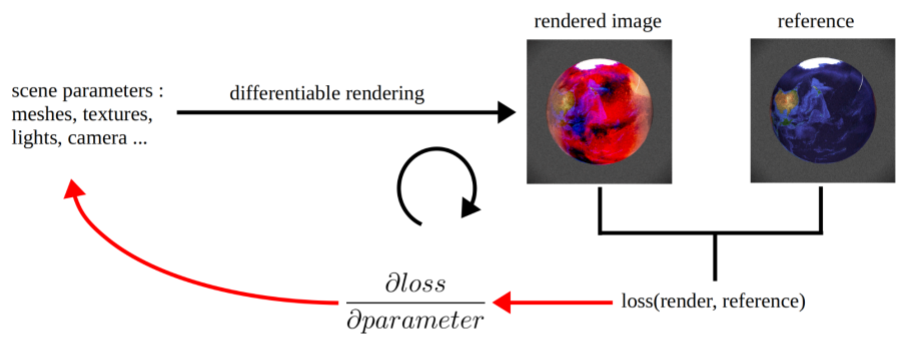
\includegraphics[width=\textwidth]{images/diffrender.png}
  \caption{Differentiable Rendering \parencite{diffrenderweb}}
  \label{diffrender}
\end{figure}

\newpage
\subsection{Background and Related Work: Pranav Talluri}

The key literature for this project is \emph{Soft Rasterizer: A Differentiable Renderer for Image-based 3D Reasoning} \parencite{softras}. The paper introduces a novel approach to differentiable rendering, replacing the standard discrete rasterisation process with a new soft rasteriser as discussed in \ref{section:softraspipealgo}. We specifically investigate the usage of the differentiable renderer to perform inverse rendering. Figure \ref{softrasresults} shows the fitting procedure, which is discussed further in \ref{section:softrasalgo}.

\begin{figure}[h!]
  \centering
  \begin{subfigure}{0.45\textwidth}
    \centering
    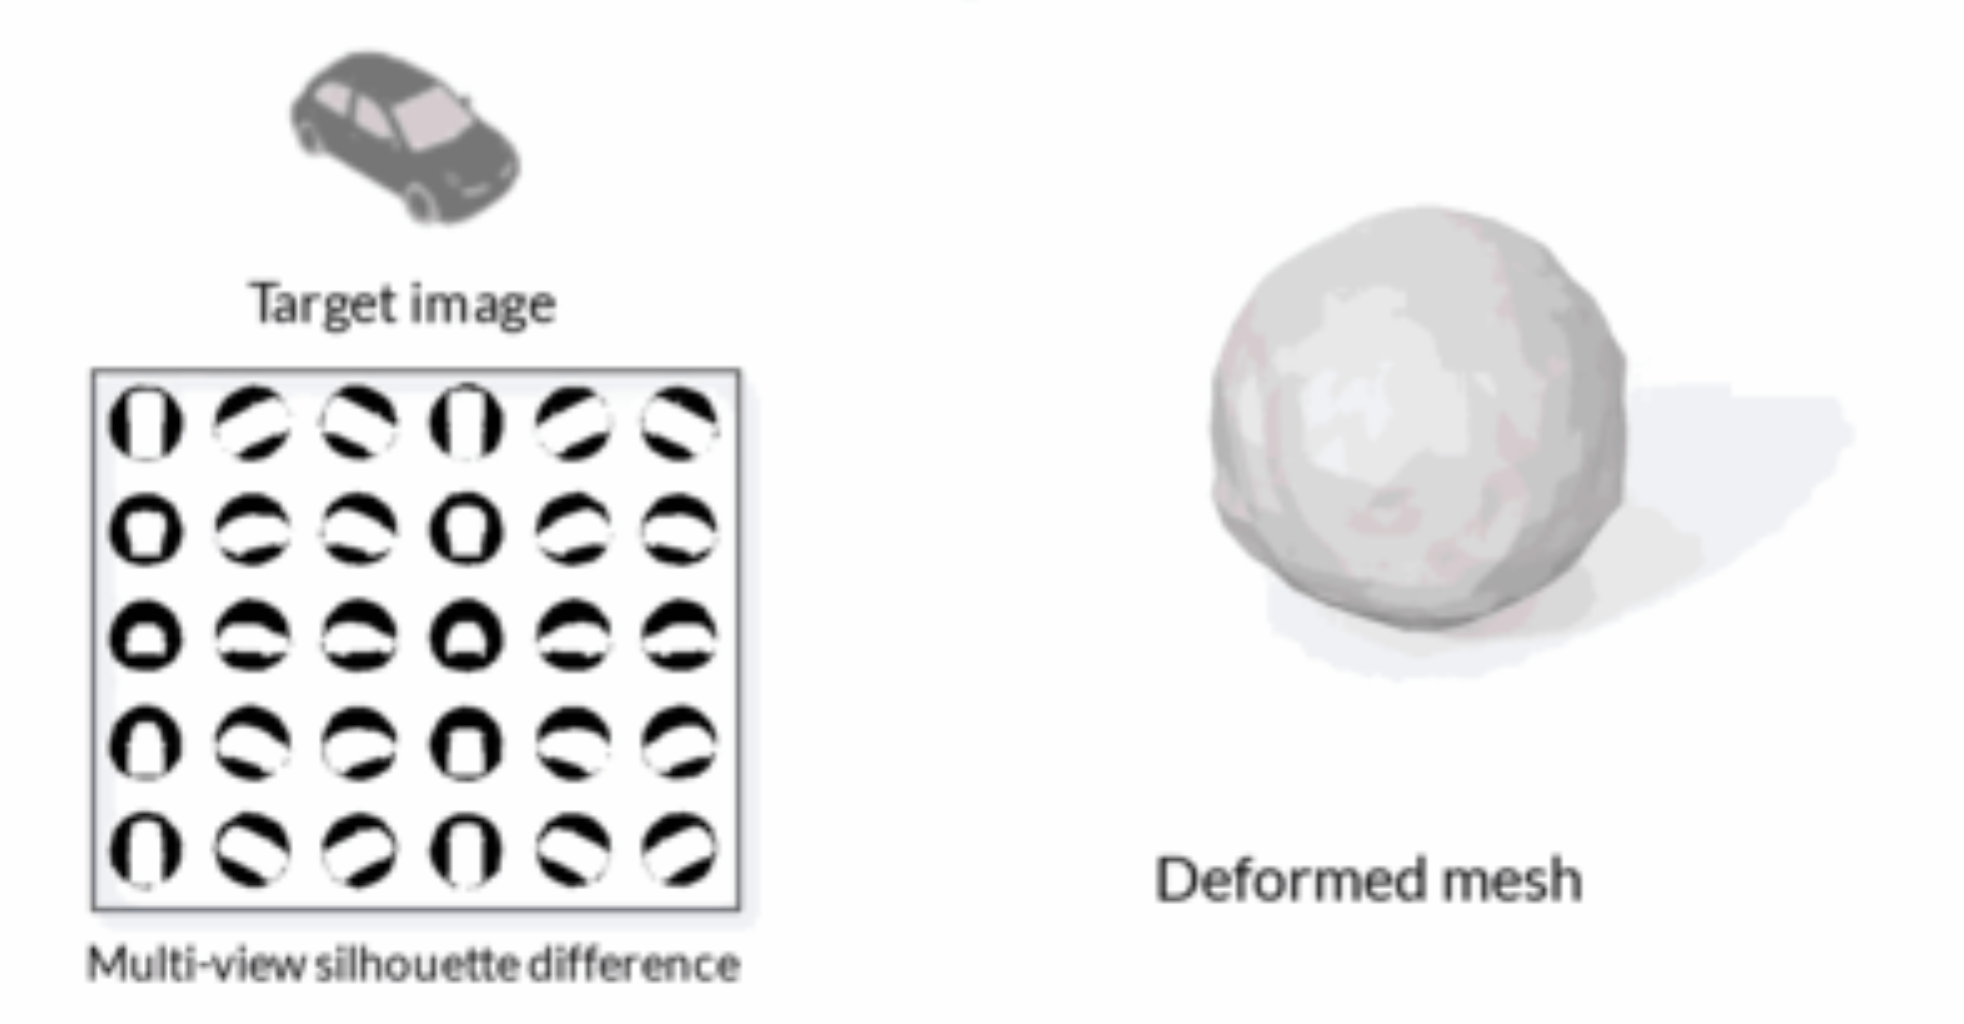
\includegraphics[width=\textwidth]{images/softrasinit.png}
    \caption{Start}
    \label{softrasstart}
  \end{subfigure}
  \hfill
  \begin{subfigure}{0.45\textwidth}
    \centering
    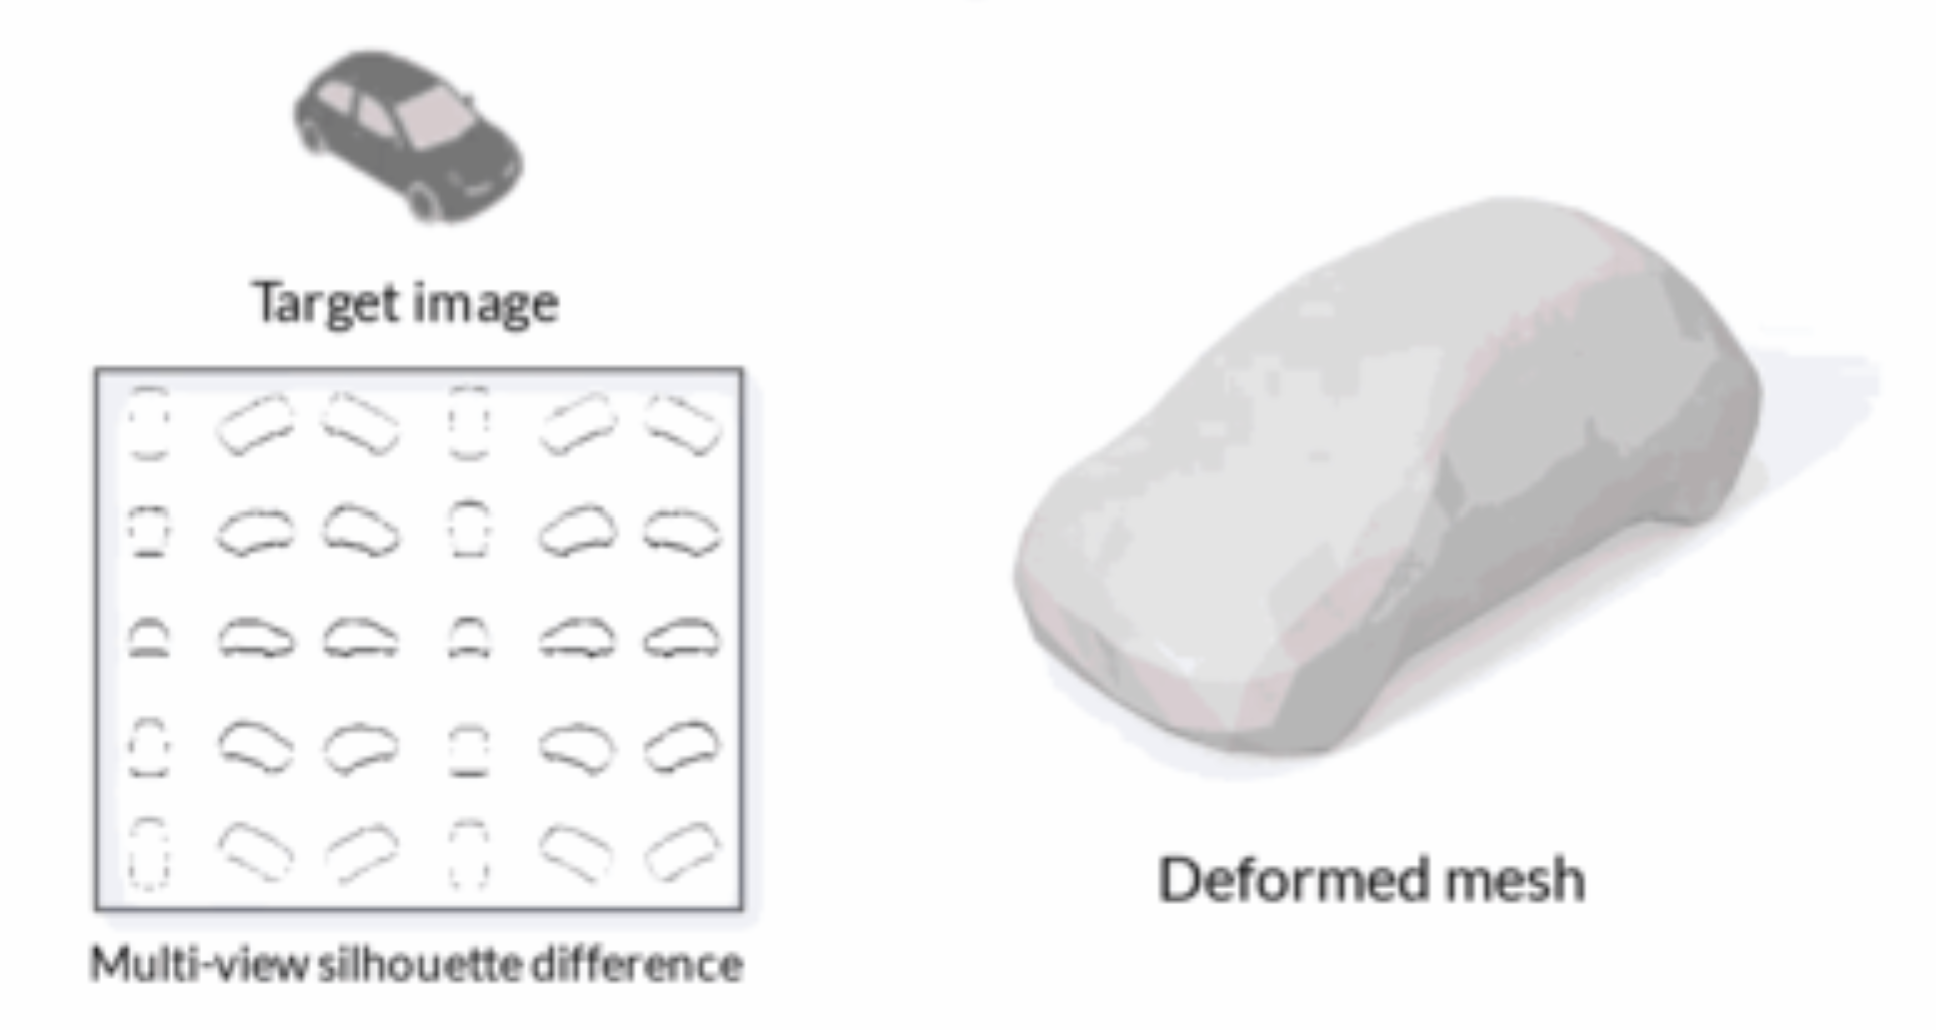
\includegraphics[width=\textwidth]{images/softrasresults.png}
    \caption{End}
    \label{softrasend}
  \end{subfigure}
  \caption{SoftRas fitting procedure \parencite{softras}}
  \label{softrasresults}
\end{figure}

Our project also uses on DeepLabv3 \parencite{deeplab} for generating image silhouettes. DeepLabv3 utilises modules which employ atrous convolution in cascade or parallel to capture multi-scale context by adopting multiple atrous rates. Atrous convolution enables adding more layers (deeper networks) without having to have larger images, as shown in Figure \ref{deeplabatrousnoatrous}. It utilises pyramid pooling modules to probe convolutional features at multiple scales.

\begin{figure}[h!]
  \centering
  \begin{subfigure}{\textwidth}
    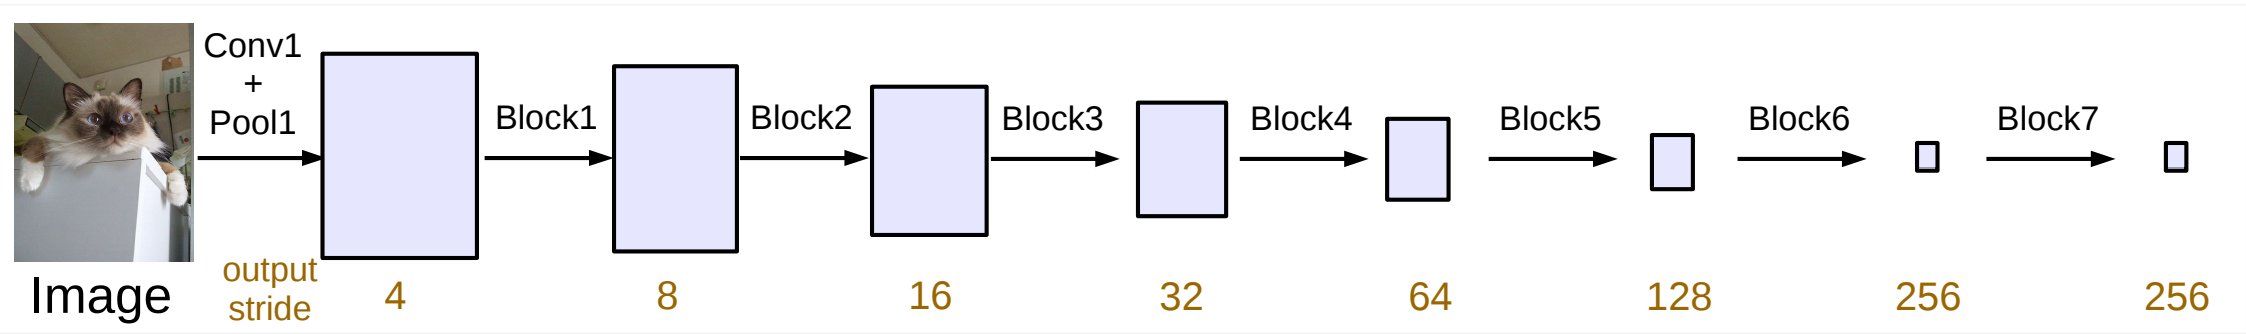
\includegraphics[width=\textwidth]{images/deeplabnoatrous.png}
    \caption{Without atrous convolutions}
    \label{deeplabnoatrous}
  \end{subfigure}
  \begin{subfigure}{\textwidth}
    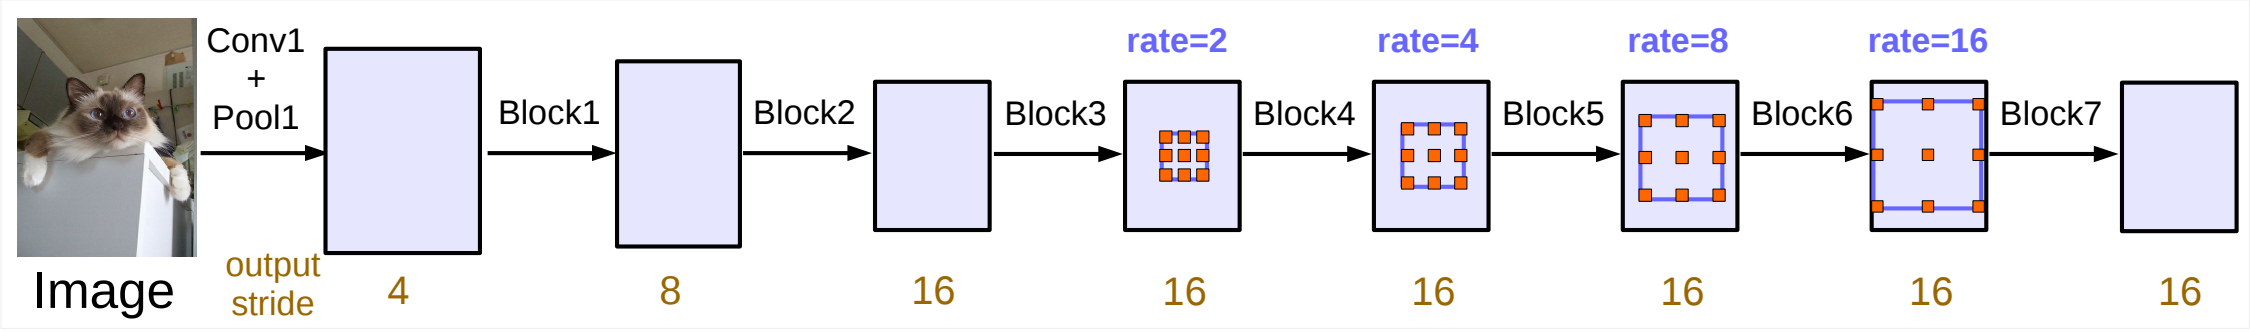
\includegraphics[width=\textwidth]{images/deeplabatrous.png}
    \caption{With atrous convolutions}
    \label{deeplabatrous}
  \end{subfigure}
  \caption{Cascaded modules and atrous convolutions \parencite{deeplab}}
  \label{deeplabatrousnoatrous}
\end{figure}

DeepLab is able to generalise well to new images due to its large and varied training dataset. The authors of the original paper also detail the typical failure modes. The model is able to perform extremely well on images with clear subjects but is weaker when given images without a clear view of the subject or differentiating between similar subject classes. The latter failure mode is not a concern for our usage of DeepLab. Some sample results are shown in Figure \ref{deeplabresults} where the first two rows show successful results and the last row visualises the failure modes.

\begin{figure}[h!]
  \centering
  \begin{subfigure}{\textwidth}
    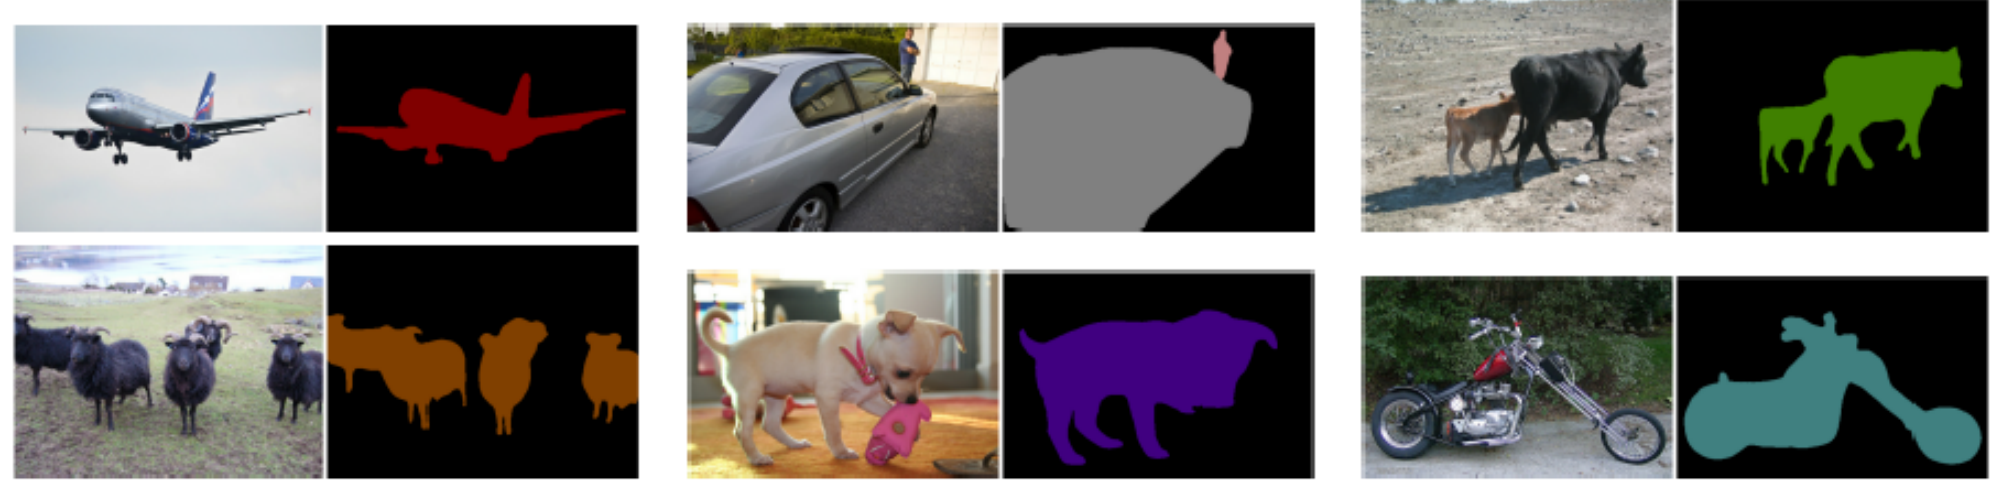
\includegraphics[width=\textwidth]{images/deeplabresultsgood.png}
    \caption{Good results}
    \label{deeplabresultsgood}
  \end{subfigure}
  \begin{subfigure}{\textwidth}
    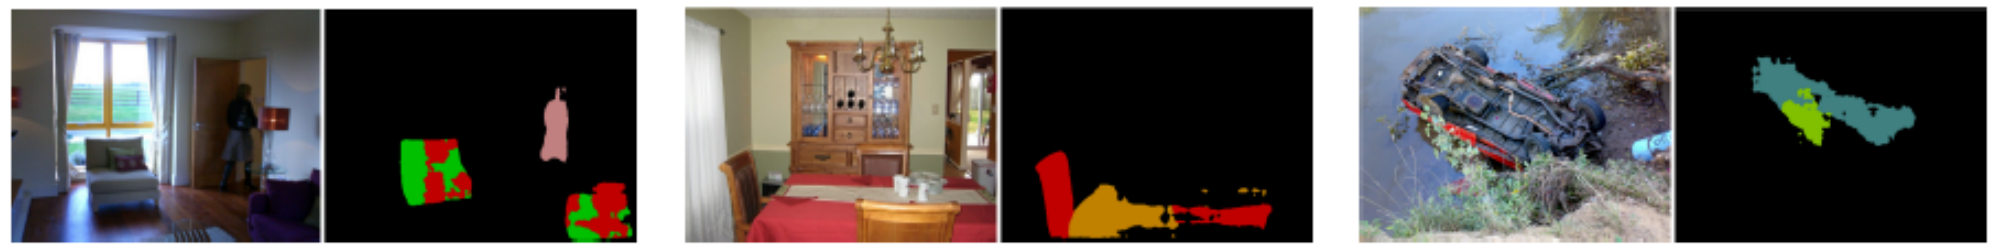
\includegraphics[width=\textwidth]{images/deeplabresultsbad.png}
    \caption{Failure modes}
    \label{deeplabresultsbad}
  \end{subfigure}
  \caption{DeepLab segmentation samples, including failure modes \parencite{deeplab}}
  \label{deeplabresults}
\end{figure}

\subsection{Overview of the Idea: Pranav Talluri}

The aim of our project is to address the initialisation of SoftRas, in order to improve its performance in constructing a fitted mesh when given images of an object from multiple viewpoints. There are three key initialisations for SoftRas which we aim to address: silhouettes, meshes and camera parameters. In addition to these initialisations, we also investigate the data used. The original paper uses a subset of the ShapeNet \parencite{shapenet} dataset, which features renders of artificial 3D models of simple objects that fit into a small number of classes.

\subsubsection{Silhouette Initialisation: Pranav Talluri}

The first initialisation is the silhouettes of the multi-view images. The original SoftRas pipeline directly takes silhouettes of the object to be reconstructed. This is possible because the authors construct renders from the ShapeNet dataset which already have a transparent background. This is problematic as most real world multi-view datasets feature full images, including a background. To address this problem, we will utilise semantic segmentation (DeepLab) to produce segmentation masks, which can then be used to generate silhouettes. Retrofitting this pipeline to SoftRas will enable us to reconstruct 3D meshes from natural 2D images.

\subsubsection{Mesh Initialisation: Pranav Talluri}

The next initialisation is the mesh that SoftRas deforms to fit to the input images. By default, the SoftRas pipeline utilises a sphere. The initial mesh has a large impact on the both the number of iterations required by the fitting procedure and the final product. We plan on modifying this initialisation based on the input images to accelerate the fitting procedure and procedure better results. The modifications are: manipulating the polygon count of the mesh, changing the scale of the sphere and translating its position.

\subsubsection{Dataset Investigation: Pranav Talluri}

The data used in the original paper comes from the ShapeNet dataset. This has some key limitations. The images utilised are relatively low resolution (64x64) and are not natural images, they come from renders of computer generated 3D models. In our project, we aim to investigate the effectiveness of SoftRas on higher resolution, photo-realistic images. We achieve this primarily by experimenting with the Amsterdam Library of Object Images (ALOI) \parencite{aloi} dataset, which contains photographic images of a large variety of objects with resolutions of 384x288. The images are also taken from more limited viewpoints (no vertical viewpoint variation), which will test the fitting procedure's ability to extend to less informative input images. This dataset includes the ground truth camera parameters, so we also aim to test the pipeline on images that we capture ourselves where the ground truth for image viewpoints is not known and the backgrounds are more challenging.

\subsubsection{Camera Parameter Initialisation: Pranav Talluri and Ke Ding}

The final initialisation is the viewpoint labels for each of the multi-view silhouettes passed as input to the fitting procedure. These parameters tell the fitting procedure which angles to generate renders of the predicted mesh from so that these renders can be compared to the silhouettes to compute a loss. The fitting procedure used in the original paper utilises ground truth viewpoint labels that are given by the ShapeNet dataset. We aim to estimate these parameters using SfM in order to enable fitting on natural images where the ground truth viewpoint parameters are unknown.

\newpage
\section{Method}
\subsection{Baseline Algorithm}
\subsubsection{Soft Rasteriser: Pranav Talluri}
\label{section:softraspipealgo}

The backbone of our project is the official implementation of SoftRas created by the authors of the paper. We utilise the soft rasteriser from this original project in order to generate renders of the predicted model. Figure \ref{softraspipe} compares the rendering pipeline used by SoftRas and a traditional pipeline.

\begin{figure}[h!]
  \centering
  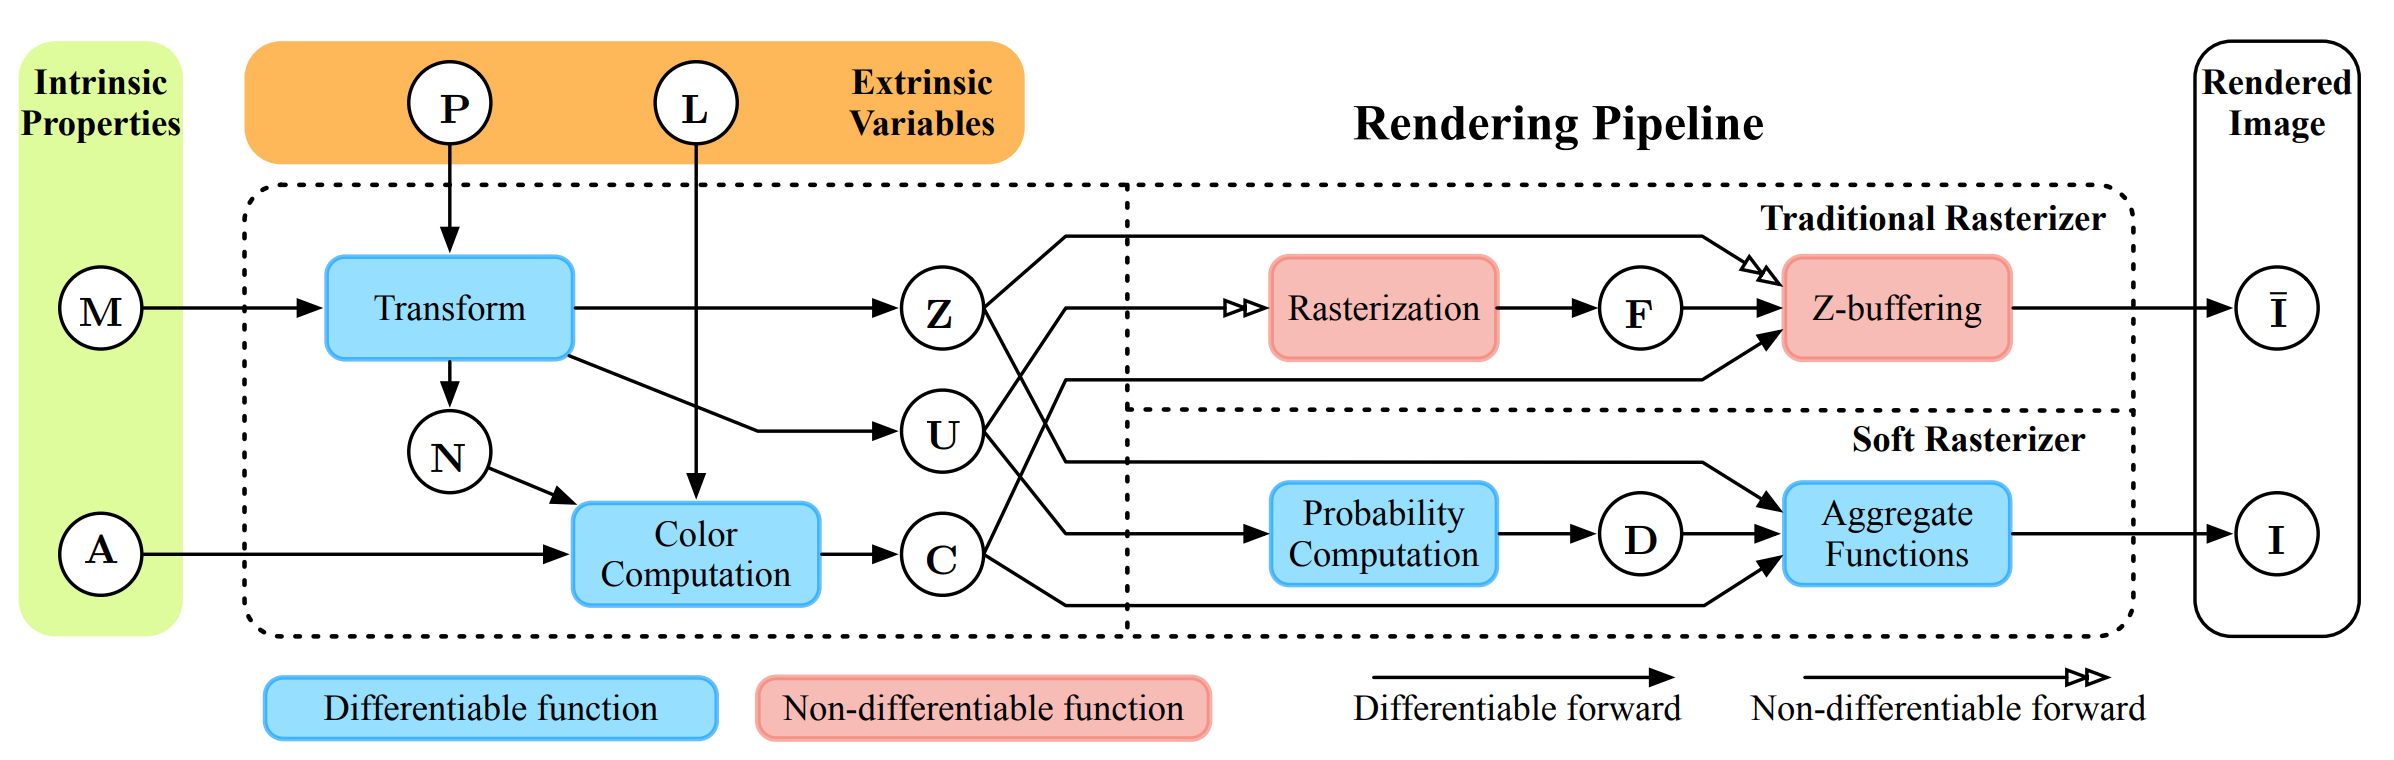
\includegraphics[width=\textwidth]{images/softraspipeline.png}
  \caption{SoftRas vs Traditional Rendering Pipeline \parencite{softras}}
  \label{softraspipe}
\end{figure}

The soft rasteriser works by aggregating probabilistic contributions from each triangle in the scene mesh, which makes it truly differentiable. This is a notable improvement over prior works in differentiable renderers, which only approximate the rendering gradient in the back propagation stage, and utilise traditional methods in the forward pass, such as \cite{neural3dmeshrenderer}. SoftRas therefore avoids an inconsistency between the forward and backward passes which would lead to uncontrolled optimisation behaviours and a limited ability to generalise to other 3D reasoning tasks.

SoftRas interprets rasterisation as a problem of binary masking determined by the relative positions between pixels and triangles, and z-buffering merges rasterisation results on a per-pixel basis using the relative depths of triangles. SoftRas then aims to solve this problem in a differentiable manner, which it achieves utilising probability maps $\{D_j\}$ and an aggregation function $A$. $D_j$ models the influence of triangle mesh $f_j$ on the image plane. We need to estimate this value using a function, which needs to take into account the relative position and distance between the pixel $p_i$ and triangle $f_j$. We define $D_j^i$ using the sigmoid function \[D^i_j = sigmoid(\delta^i_j \times \frac{d^2(i,j)}{\sigma})\text{.}\]

For each mesh triangle $f_j$, we define its colour map $C_j$ at pixel $p_i$ on the image plane by interpolating vertex colour using barycentric coordinates.

$A$ is an aggregate function that we use to merge the colour maps $\{C_j\}$ and obtain rendering output $I$ based on probability maps $\{D_j\}$ and the relative depths $\{z_j\}$. Figure \ref{softrasraster} shows how this compares with a traditional, discrete rasterisation pipeline.

\begin{figure}[h!]
  \centering
  \begin{subfigure}{.49\textwidth}
    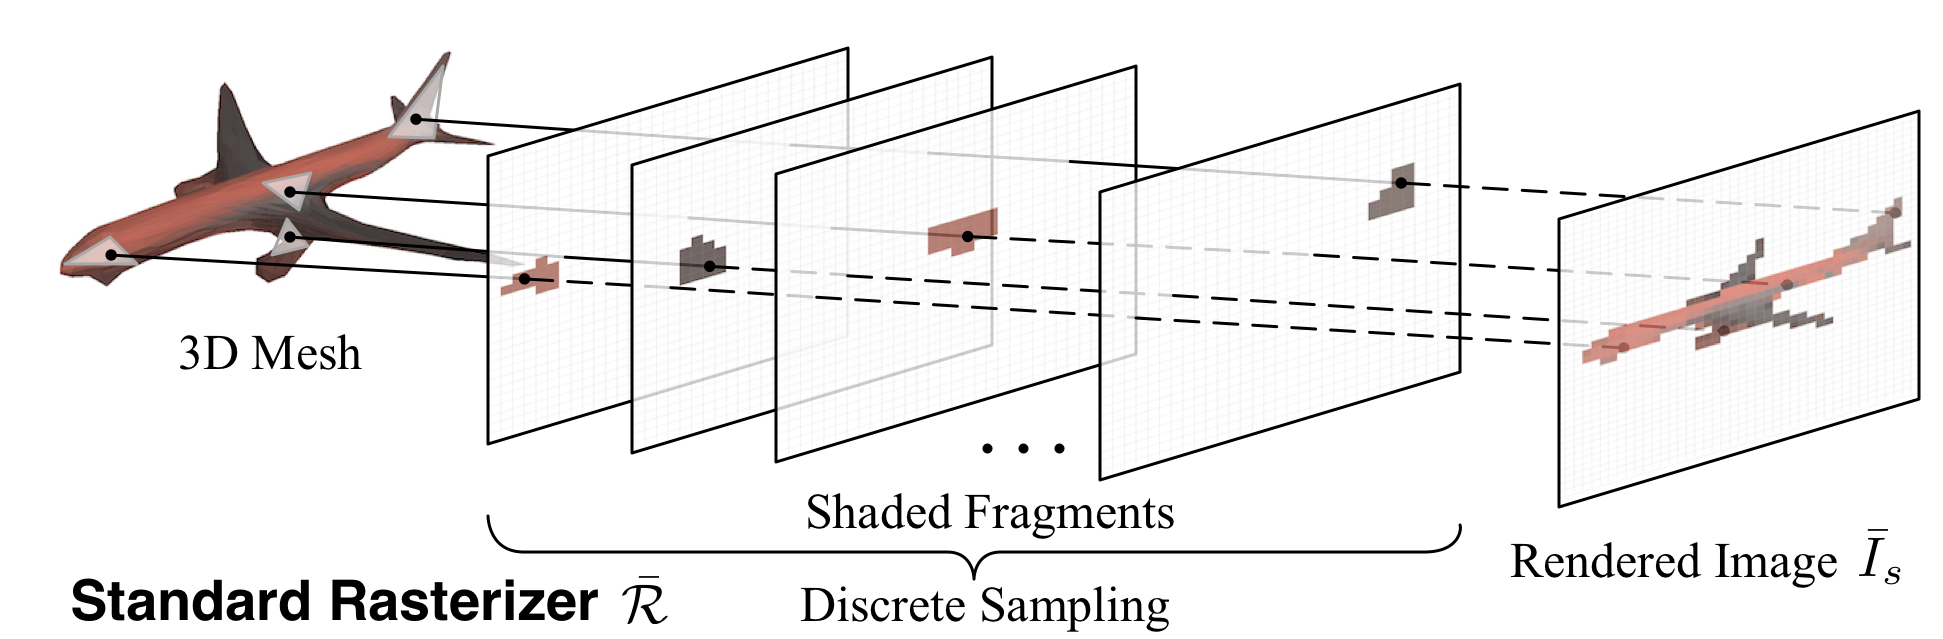
\includegraphics[width=\textwidth]{images/softras_b.png}
    \caption{Traditional rasteriser}
    \label{trad}
  \end{subfigure}
  \begin{subfigure}{.49\textwidth}
    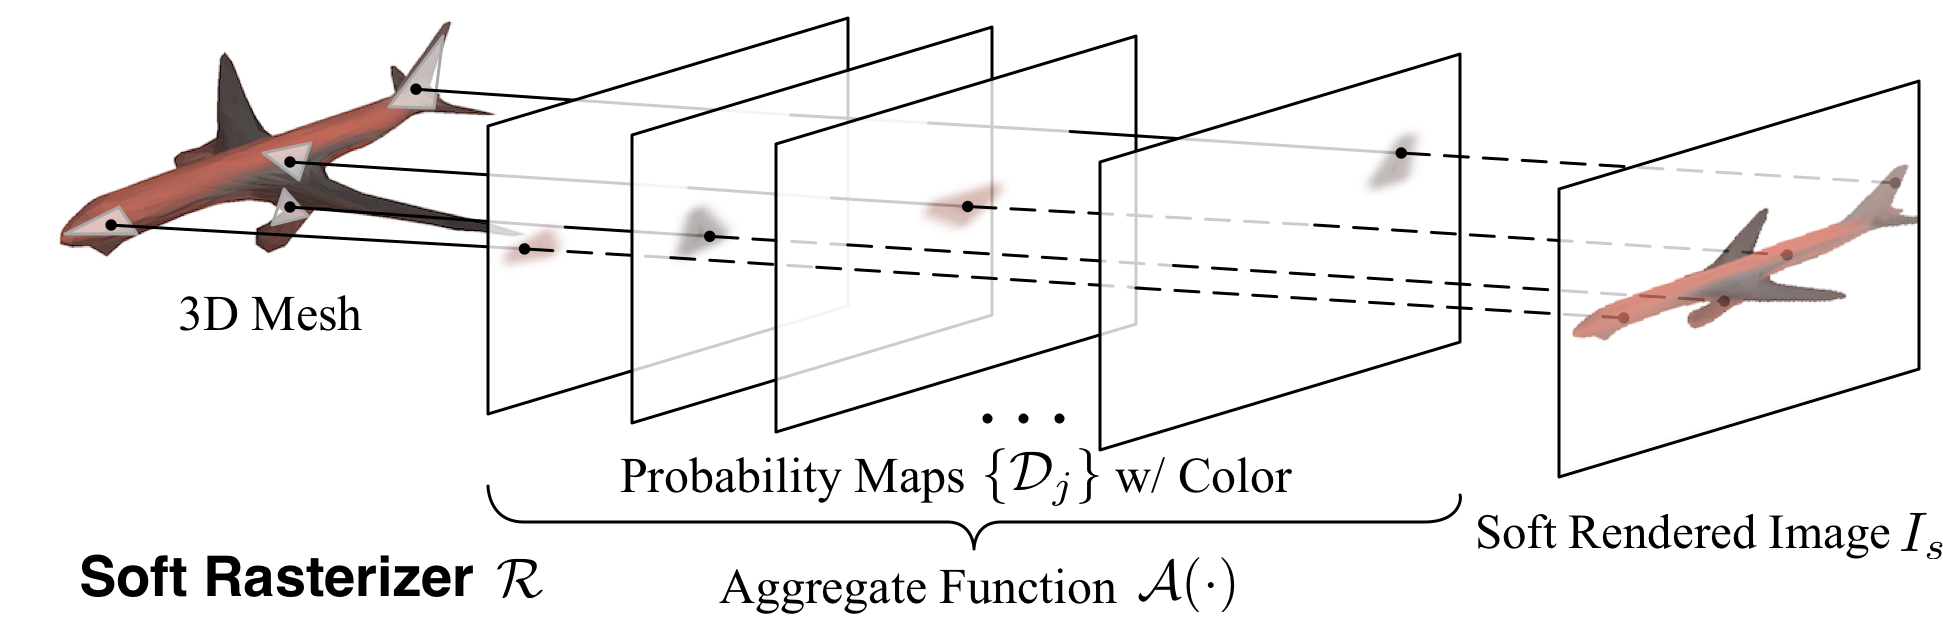
\includegraphics[width=\textwidth]{images/softras_a.png}
    \caption{Soft Rasteriser}
    \label{soft}
  \end{subfigure}
  \caption{Traditional vs Soft Rasteriser \parencite{softras}}
  \label{softrasraster}
\end{figure}

\subsubsection{Fitting Procedure: Pranav Talluri}
\label{section:softrasalgo}
Given an initial mesh, the procedure makes changes to the faces and vertices of the mesh, produces 2D renders of this mesh using the soft rasteriser and then compares these renders to the input images to compute a loss. This loss is then used to inform back-propagation through the rendering pipeline to modify the mesh. This repeats for some large number of iterations. The initial mesh, therefore, has a large impact on the performance of the process, including the number of iterations required to converge, the mesh that is converged at and whether or not the procedure is able to converge.

The loss is computed using the intersection over union (IoU) between the renders and the input images. This is a common choice for measuring similarity between images. We are unable to use 3D IoU using voxels as we do not have a ground truth 3D model of the target object, so we approximate with 2D IoU averaged over all the viewpoints. Given a set of $n$ ground truth images $i_{gt}$, viewpoints $v_{gt}$ and a predicted mesh $m_{pred}$, we generate projections $i_{pred}$ of $m_{pred}$ at $v_{gt}$ using SoftRas. We specifically compute the loss as a negation of the average IoU over the multiple viewpoints: \[IoU = 1 - \frac{1}{n}\sum_{j=0}^n\frac{intersection(i_{gt, j}, i_{pred, j})}{union(i_{gt, j}, i_{pred, j})}\]

\subsubsection{Data: Pranav Talluri}
Originally, SoftRas directly takes multi-view silhouettes as an input. The pipeline requires a 4 channel image (R, G, B and Alpha for transparency), so it doesn't support standard RGB images. If given an RGBA image with no transparent regions, the fitting procedure is not able to properly generate a mesh for the subject of the image as the transparency is required for loss computation. i.e., The transparent regions of the images tell SoftRas which regions to treat as the background. Figure \ref{shapenetdatapipe} shows the data pipeline used by the original implementation of the fitting procedure. An example of an input to the original pipeline taken from ShapeNet renders is shown in Figure \ref{shapenetinput}

\begin{figure}[h!]
  \centering
  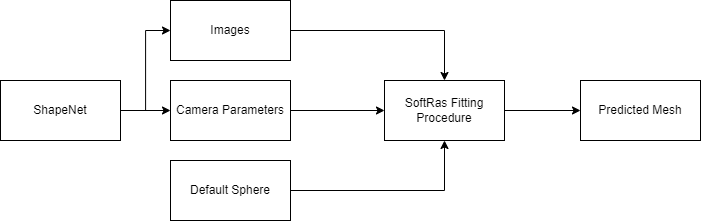
\includegraphics[width=\textwidth]{images/shapenetdatapipe.png}
  \caption{Data pipeline of original project}
  \label{shapenetdatapipe}
\end{figure}

\begin{figure}[h!]
  \centering
  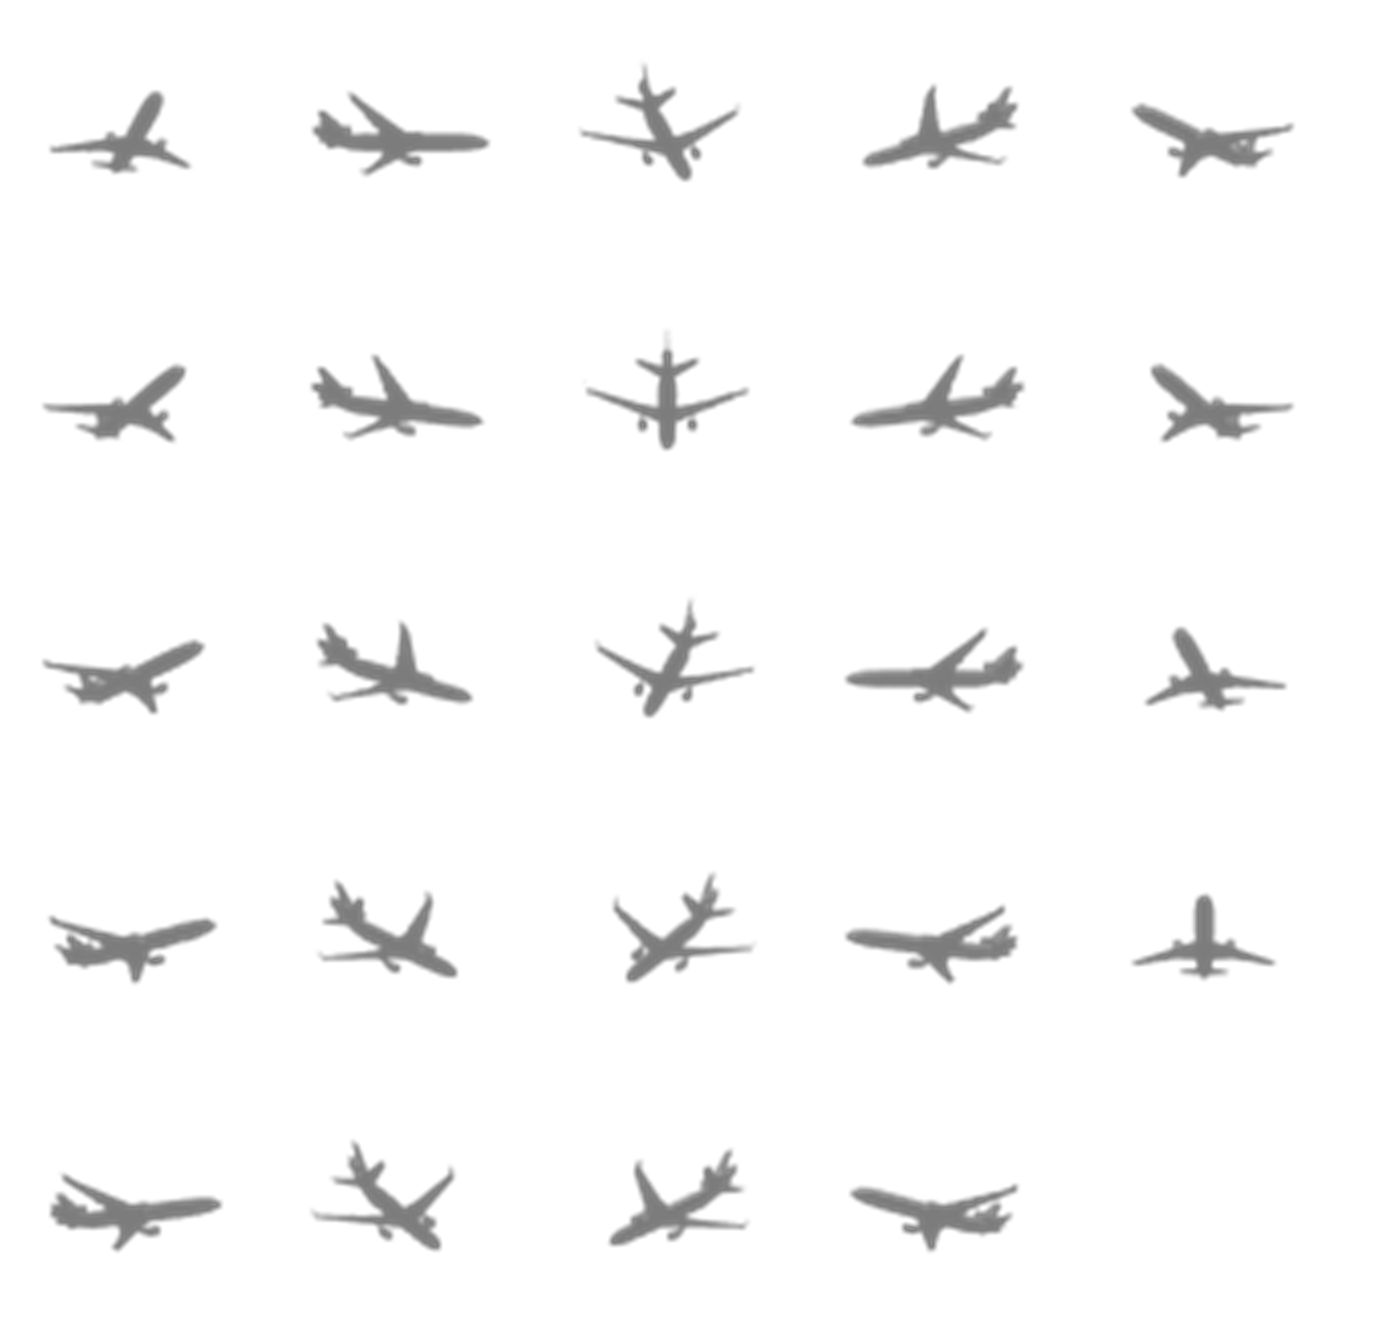
\includegraphics[width=0.5\textwidth]{images/shapenetinput.png}
  \caption{Silhouette Input from ShapeNet renders}
  \label{shapenetinput}
\end{figure}

The pipeline takes images with a 64x64 resolution, but it is extensible to other (square) resolutions. However, attempting to use much higher resolution images produces poor results, qualitatively and quantitatively, but the speed of the fitting procedure is the real limiting factor. The pipeline also takes a camera viewpoint for every image. This determines which directions the fitting procedure should generate renders of the mesh from to compute a loss between the input images and the renders.

\subsection{Algorithm Improvements}
\subsubsection{Data: Pranav Talluri}
The original pipeline is built for images from ShapeNet. In order to utilise other data sources, we first build a pipeline for processing input images. We modify SoftRas to operate on 256x256 input images. We then resize all larger input images to this size. Details for how these images are converted to silhouettes are in \ref{section:silimp}. We also need to make adjustments to the mesh to deal with the more detailed images and the details for this are in \ref{section:meshimp}.

To investigate the performance of SoftRas on higher resolution, photo-realistic data, we utilise the Amsterdam Library of Objects (ALOI) dataset \parencite{aloi}. It contains images of 1000 small objects at a resolution of 384 x 288. We test these changes using both ALOI, where the camera parameters and silhouettes are known, and images that we have captured, where we have no viewpoint or silhouette ground truth. Some sample images from ALOI are shown in Figure \ref{aloisamples}. Some sample images that we captured are shown in Figure \ref{natsamples}.

\begin{figure}[h!]
  \centering
  \begin{subfigure}{0.45\textwidth}
    \centering
    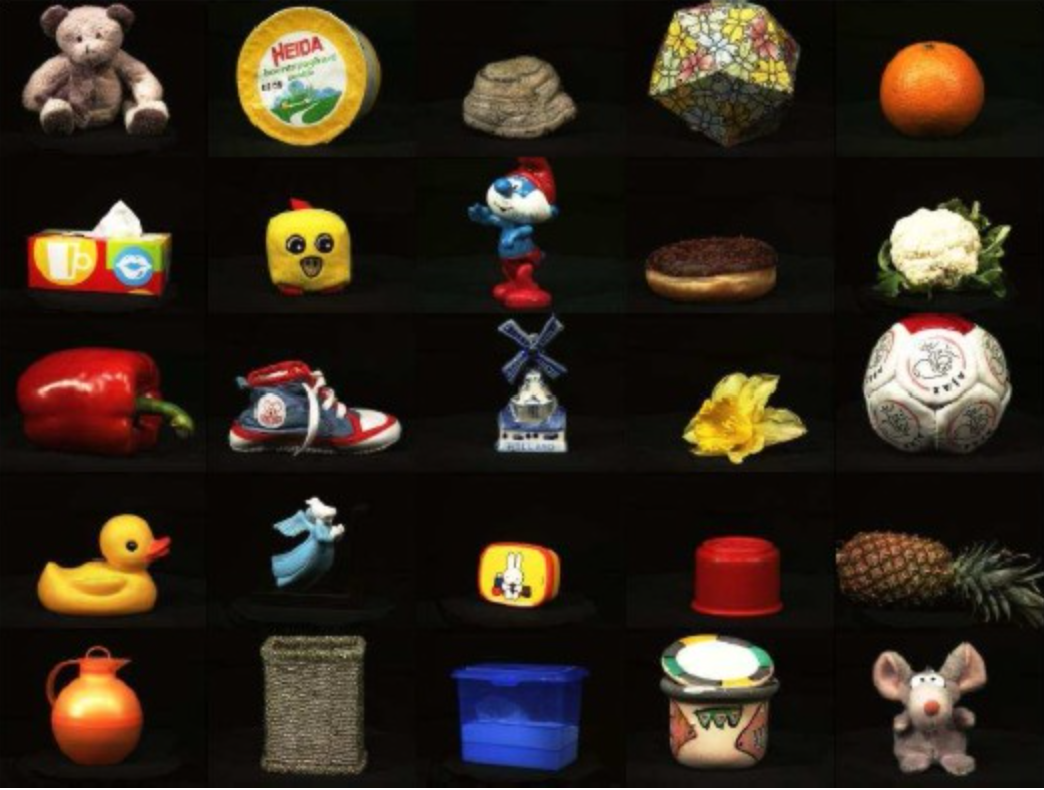
\includegraphics[width=\textwidth]{images/aloiobjects.png}
    \caption{Sample of different objects}
    \label{aloiobjects}
  \end{subfigure}
  \hfill
  \begin{subfigure}{0.45\textwidth}
    \centering
    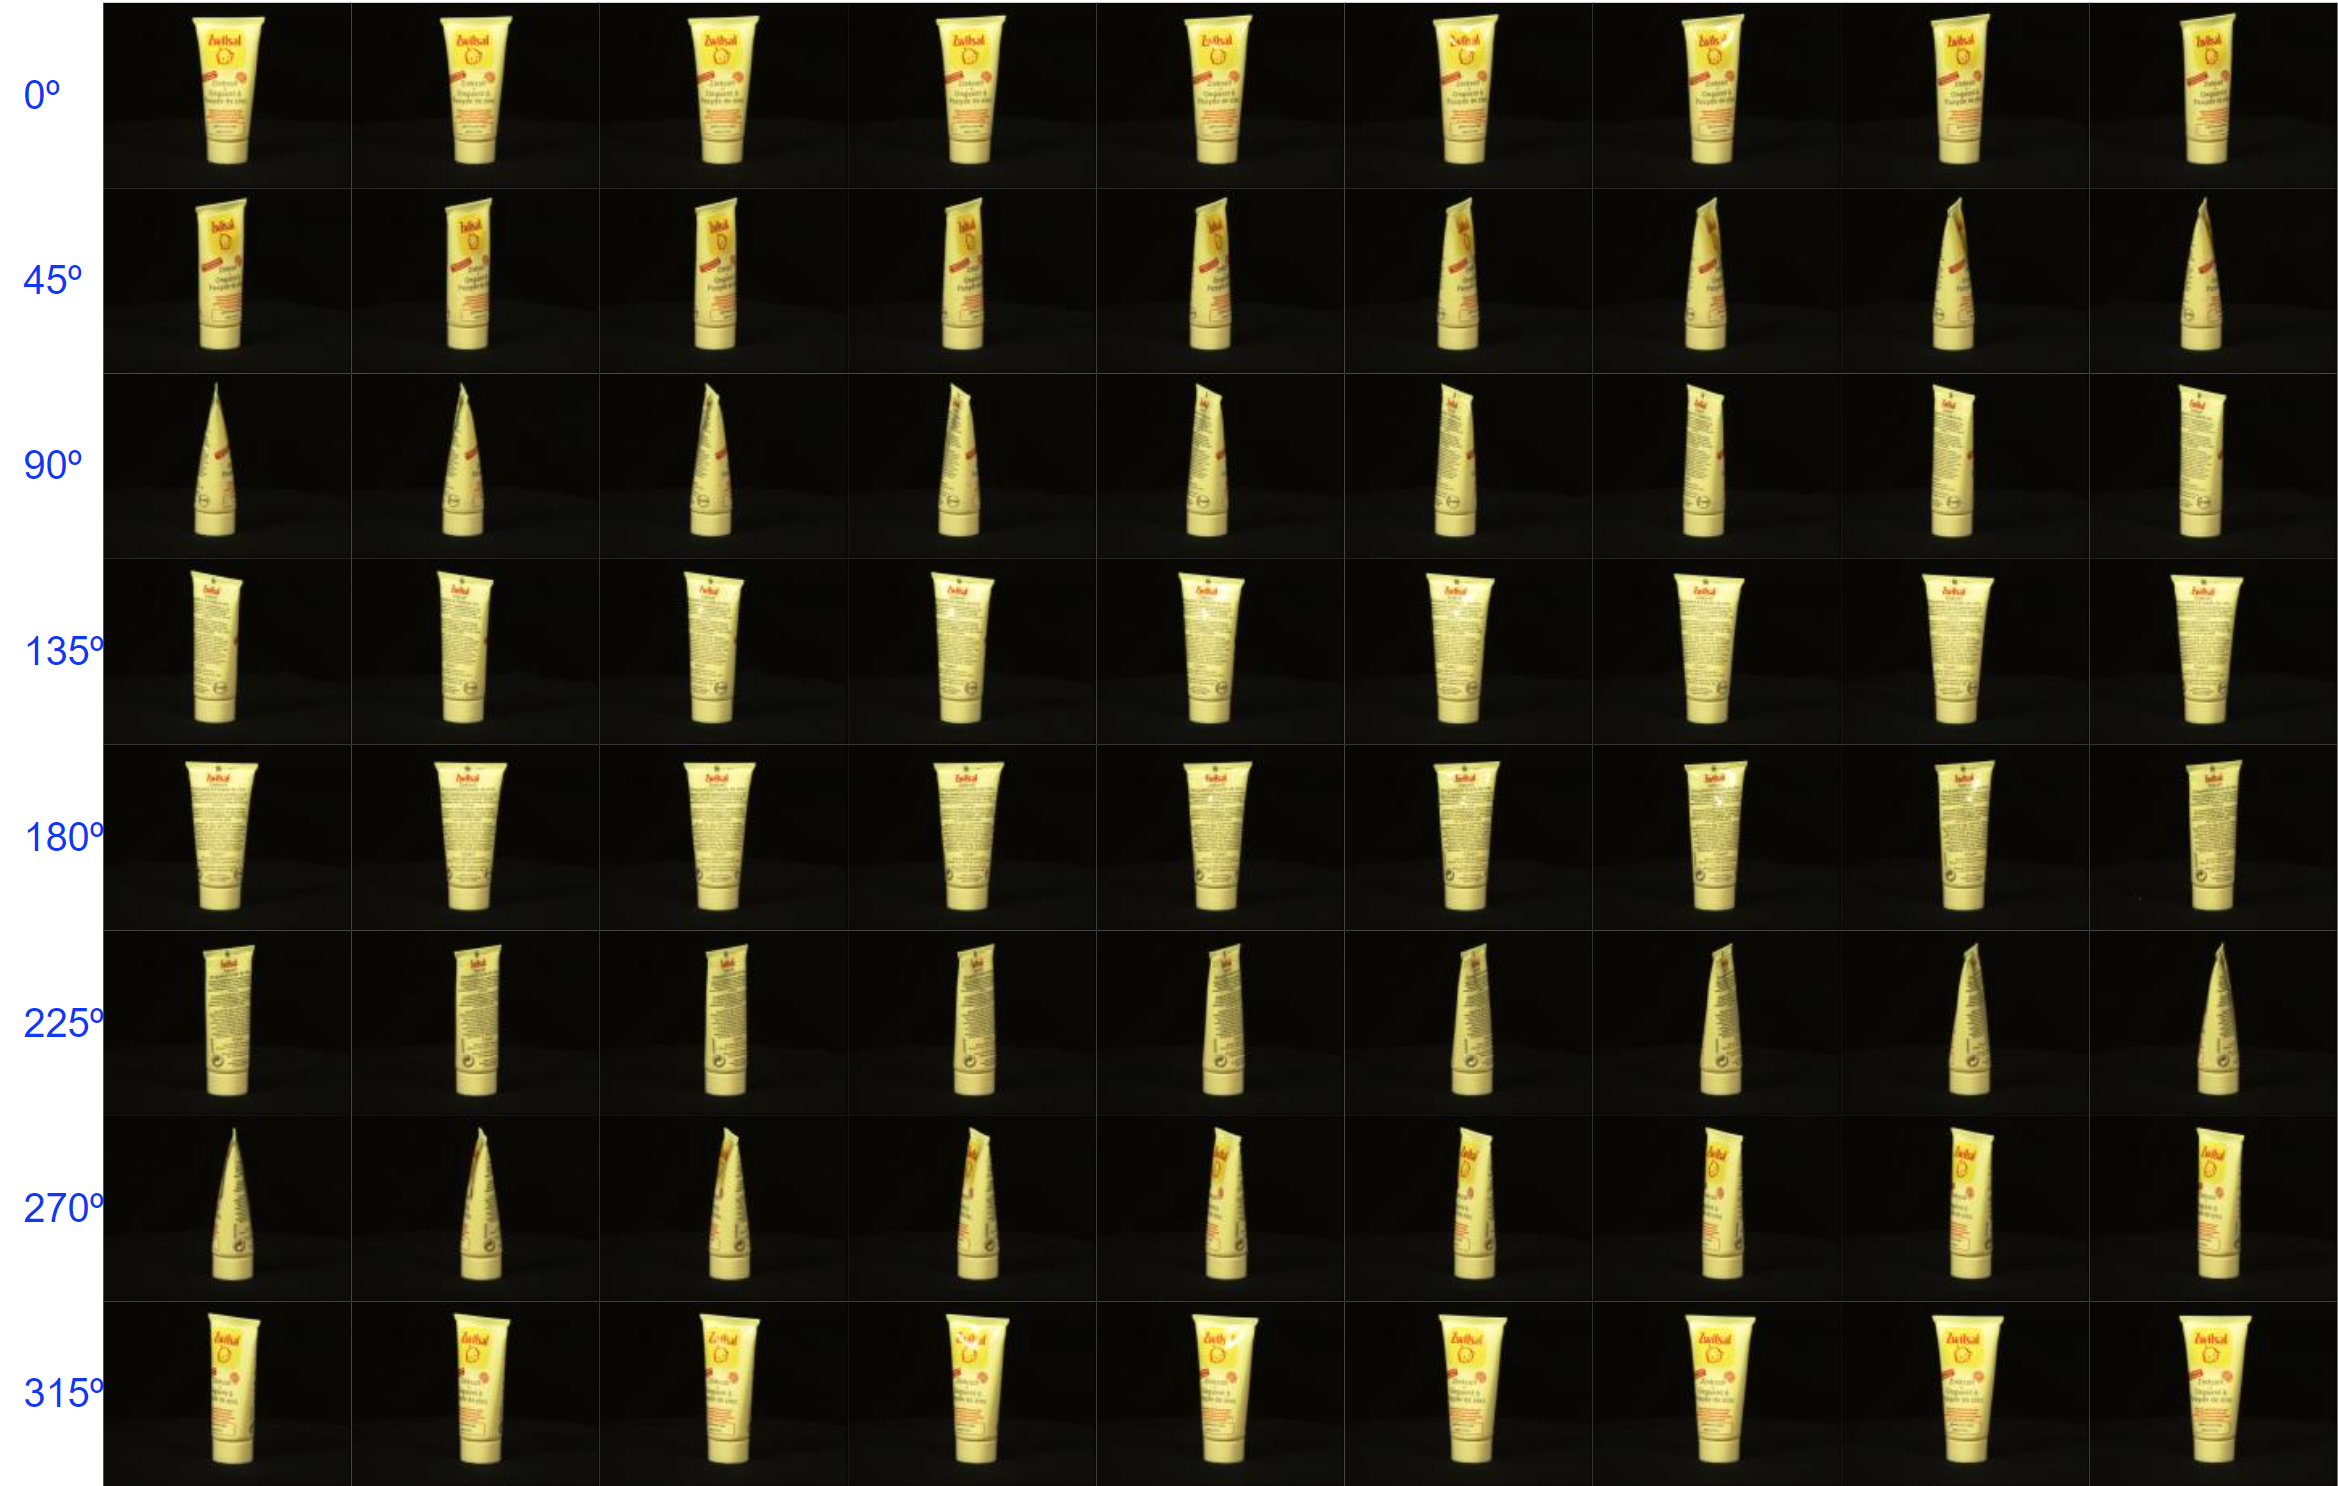
\includegraphics[width=\textwidth]{images/aloiviews.png}
    \caption{Each object is captured from 72 angles}
    \label{aloiviews}
  \end{subfigure}
  \caption{Samples from ALOI dataset.}
  \label{aloisamples}
\end{figure}

\begin{figure}[h!]
  \centering
  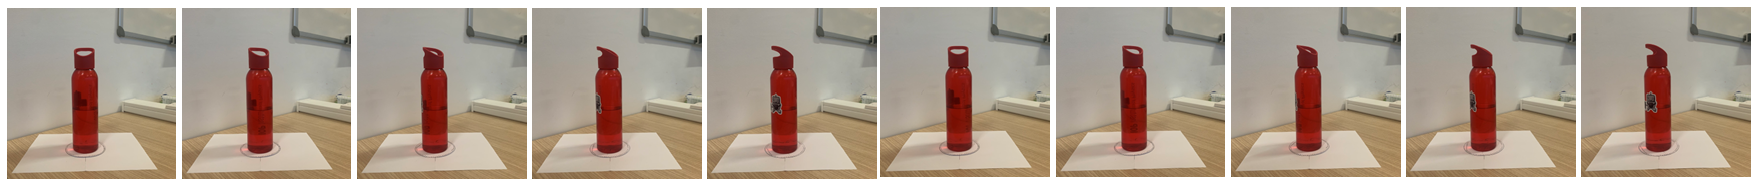
\includegraphics[width=\textwidth]{images/natsamples.png}
  \caption{Samples of natural images that we captured}
  \label{natsamples}
\end{figure}

\subsubsection{Silhouette Initialisation: Pranav Talluri}
\label{section:silimp}

Synthetic datasets such as ShapeNet allow us to directly produce silhouettes. For carefully produced photo-realistic datasets such as ALOI, where object/background mask labels have been provided, silhouettes can be generated as shown in \ref{section:datapipe}. However, for natural images, these silhouettes have to be estimated.

We modify the pipeline to enable fitting meshes for natural images with backgrounds. We utilise DeepLabv3, to produce a segmentation map of a set of inputs. We can then convert the semantic classifications into a binary pixel map, with 0 representing the background and 1 representing the subject of the image. We utilise this binary pixel map as the alpha channel of the image and also to set the pixel values of the background of the image to 0. We also convert the active pixel values to grey pixels, as the colour information is not utilised. These new images can be used as silhouette inputs to the standard SoftRas pipeline.

\[
  I = 
  \begin{bmatrix}
    I_R & I_G & I_B\\
  \end{bmatrix}
\] $I_R, I_G, I_B$ are matrices with values for each pixel in image $I$.

\[deeplab(i) = C\] $C$ is a matrix of semantic classifications for each pixel.

\[M = (C > 0)\] $M$ is a matrix of binary classifications (object or background) for each pixel.

\[\alpha = M \times 255\] $\alpha$ is a matrix of alpha channel values.

\[I'_{i,j} = I_{i,j} * (M_{i,j} \times 124)\] $I'$ is a grey-scale version of $I$ with zeroed background pixels.

\[
  I_{out} =  
  \begin{bmatrix}
    I'_R & I'_G & I'_B & \alpha\\
  \end{bmatrix}
\]

\subsubsection{Mesh Initialisation: Pranav Talluri}
\label{section:meshimp}
We modify the initial mesh passed to the fitting procedure. The sphere used in the original pipeline, shown in Figure \ref{sphereinit}, has some key issues.

A fixed size sphere is used, so if the images provided detail a subject that is much larger or smaller than the sphere, then many iterations are used to adjust the size of the mesh, if it succeeds at all. Figure \ref{apricottarget} shows an example where the position and scale of the target (a small apricot at the bottom of the image) leads to failure with the sphere initialisation. To address this, we vary the size of the initial mesh based on the input images as well as scaling the $x$ and $y$ dimensions to match the aspect ration of the target object. We do this by forming a bounding box around the target object and calculating the scale factor to modify the height and width of the sphere by accordingly. The equation below hides the complexity of converting between pixel based widths for the target image and real-world measurement units for the sphere.

\[w_{scale} = \frac{w_{sphere}}{w_{target}} ;\; h_{scale} = \frac{h_{sphere}}{h_{target}}\]

\begin{figure}[h!]
  \centering
  \begin{subfigure}{0.3\textwidth}
    \centering
    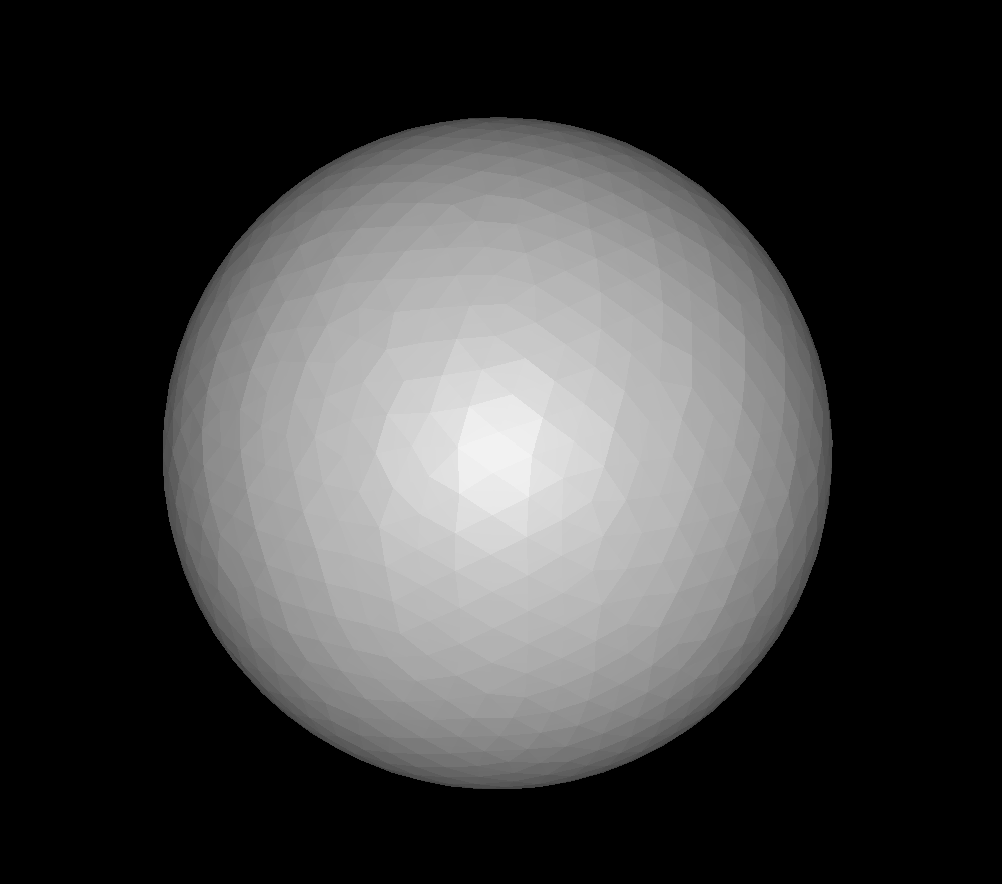
\includegraphics[width=\textwidth]{images/sphereinit.png}
    \caption{Sphere-based mesh initialisation}
    \label{sphereinit}
  \end{subfigure}
  \hfill
  \begin{subfigure}{0.3\textwidth}
    \centering
    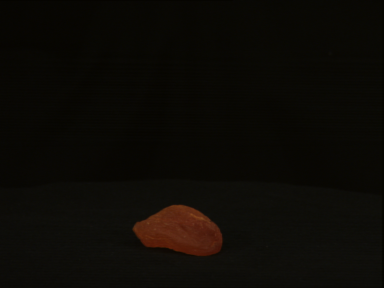
\includegraphics[width=\textwidth]{images/apricot.png}
    \caption{Target object: an apricot}
    \label{apricot}
  \end{subfigure}
  \hfill
  \begin{subfigure}{0.25\textwidth}
    \centering
    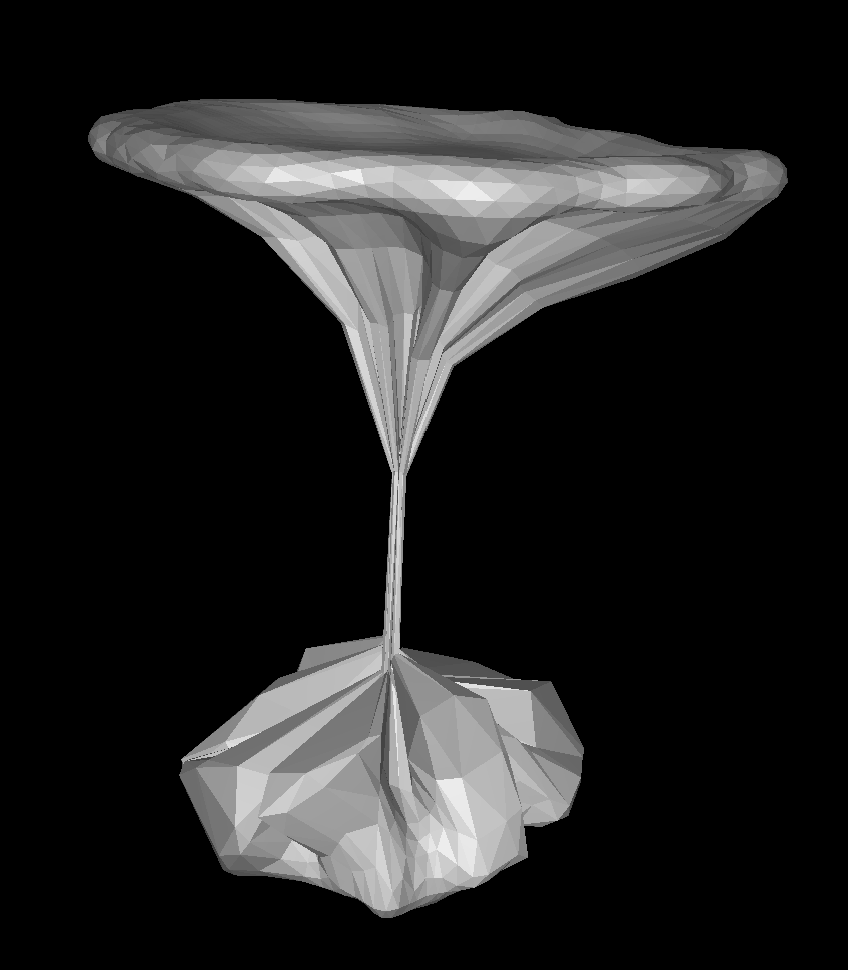
\includegraphics[width=\textwidth]{images/apricotfailure.png}
    \caption{Failure to converge}
    \label{apricotfailure}
  \end{subfigure}
  \caption{Failure to converge with sphere initialisation}
  \label{apricottarget}
\end{figure}

Another issue is that the sphere is always centred at the origin. This is not an issue for synthetic datasets like SoftRas, where the target object is likely at the centre of the frame. However, for photo-realistic datasets such as ALOI, and especially for natural images captured by a camera/phone, the subject is unlikely to be centred at the origin. This means that the fitting procedure will utilise many iterations to move the mesh to where the subject is within the image. Additionally, this is achieved by moving individual vertices, which leads to stretching, distortion and twisting artefacts as shown in Figure \ref{buckettarget}. To address this, we translate the initial mesh according to the position of the subject within the input images. We once again achieve this using a bounding box on the target object. This step is performed after the scaling, so aligning the top and left of the sphere with the top and left of the target object is sufficient for aligning the image and mesh.

\[w_{shift} = l_{mesh} - l_{object} ;\; h_{shift} = t_{mesh} - t_{object}\]

\begin{figure}[h!]
  \centering
  \begin{subfigure}{0.4\textwidth}
    \centering
      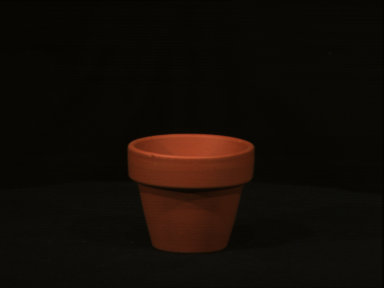
\includegraphics[width=\textwidth]{images/bucket.png}
      \caption{Target object: bucket}
      \label{bucket}
  \end{subfigure}
  \hfill
  \begin{subfigure}{0.25\textwidth}
    \centering
      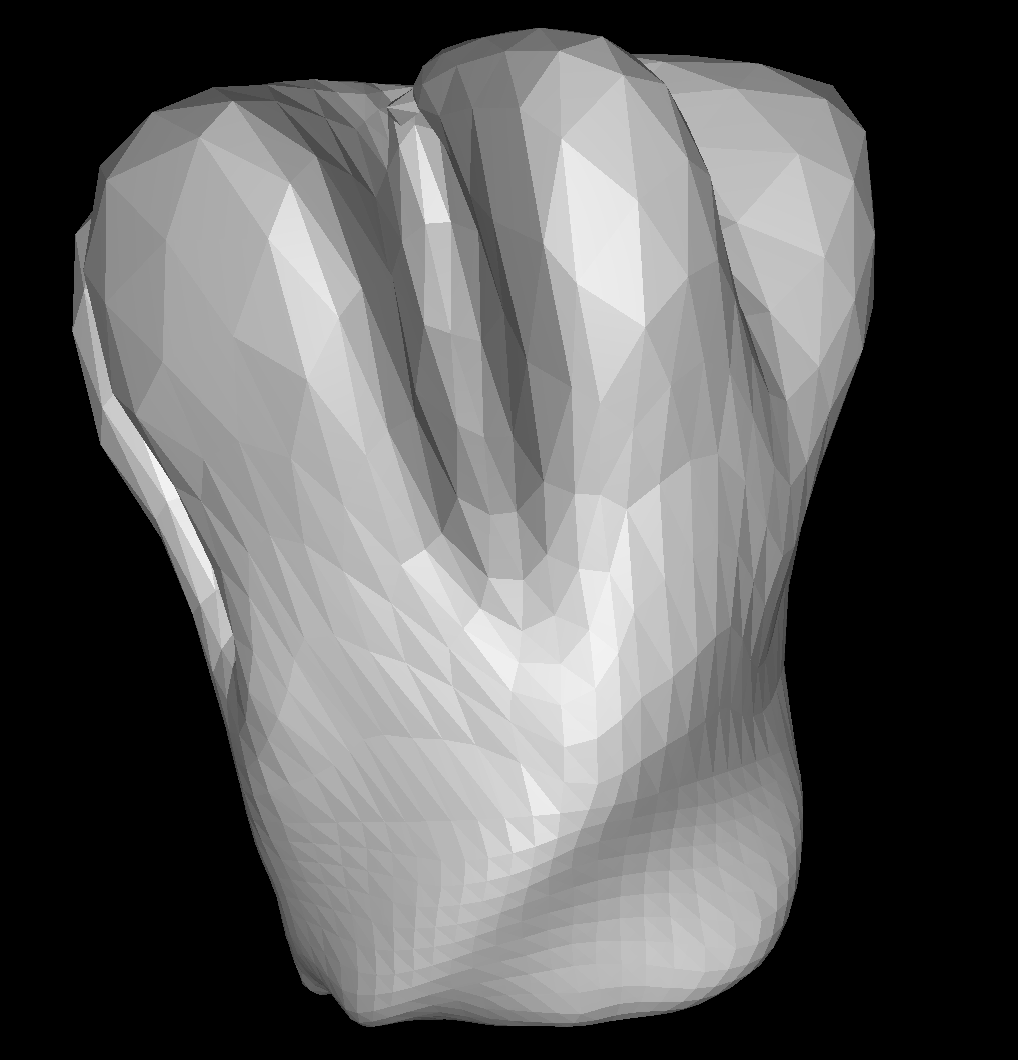
\includegraphics[width=\textwidth]{images/bucketartefact_b.png}
      \caption{Reconstruction with no mesh initialisation}
      \label{bucketfailure_a}
  \end{subfigure}
  \hfill
  \begin{subfigure}{0.25\textwidth}
    \centering
      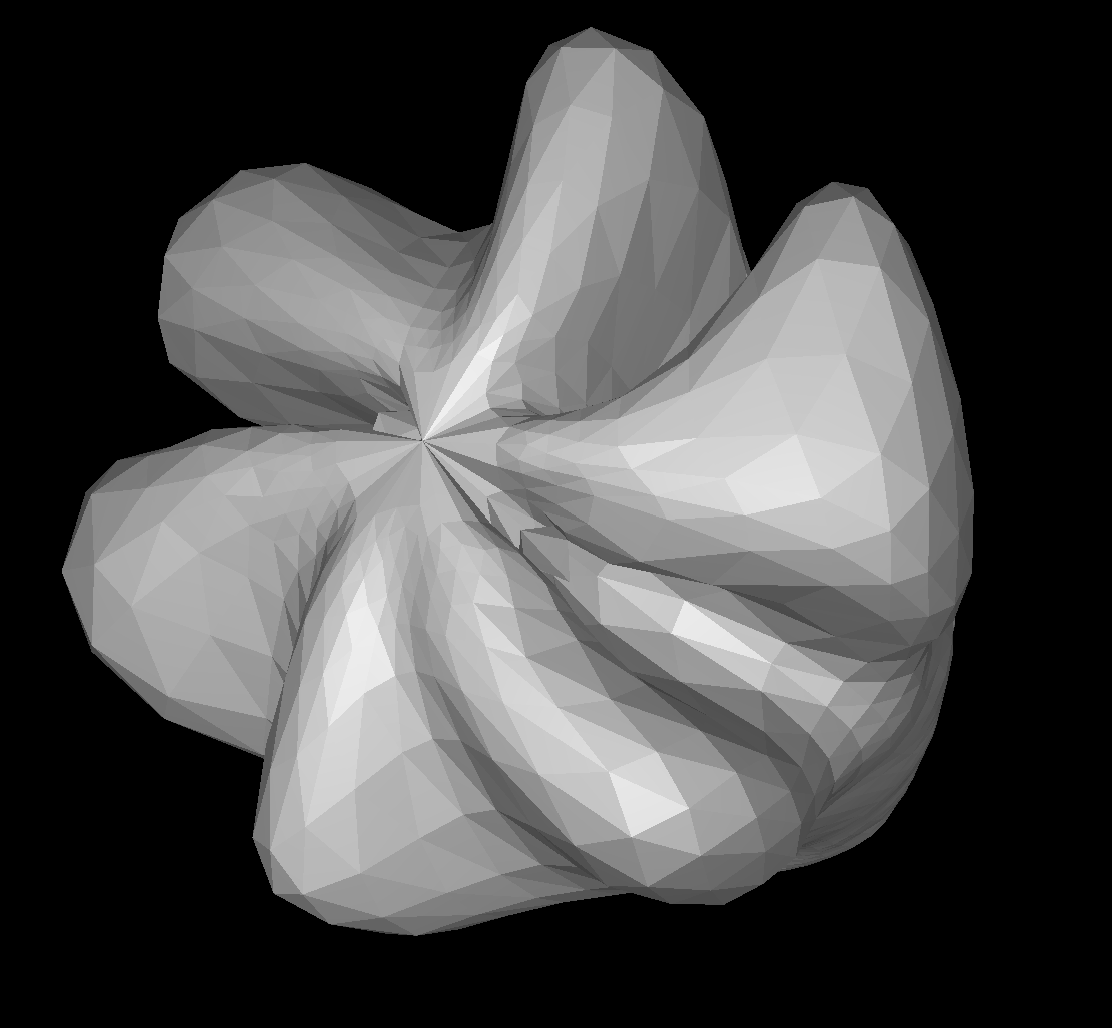
\includegraphics[width=\textwidth]{images/bucketartefact.png}
      \caption{Twisting artefacts due to off-centre target}
      \label{bucketfailure_b}
  \end{subfigure}
  \caption{Artefacts with sphere initialisation}
  \label{buckettarget}
\end{figure}

The sphere used in the original pipeline has roughly 1300 polygons. This polygon count does not vary during the fitting procedure, only the positions of the vertices. This is sufficient for the simple 64x64 images used in the original pipeline, but not for higher resolution images with more high frequency information. In Figure \ref{teddytarget}, the detail in the predicted mesh of the target is limited by the polygon count of the sphere. To address this, we introduce a new sphere with around 1900 polygons that we created in Blender and dynamically choose the initial sphere based on the target image, selecting between 600, 1300 and 1900 polygons.

\begin{figure}[h!]
  \centering
  \begin{subfigure}{0.45\textwidth}
    \centering
    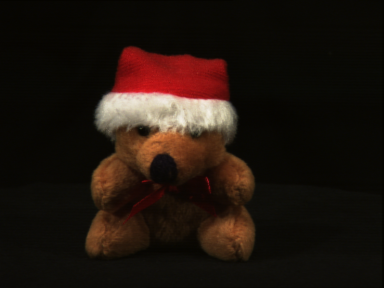
\includegraphics[width=\textwidth]{images/teddy.png}
    \caption{Target object}
    \label{teddy}
  \end{subfigure}
  \hfill
  \begin{subfigure}{0.3\textwidth}
    \centering
    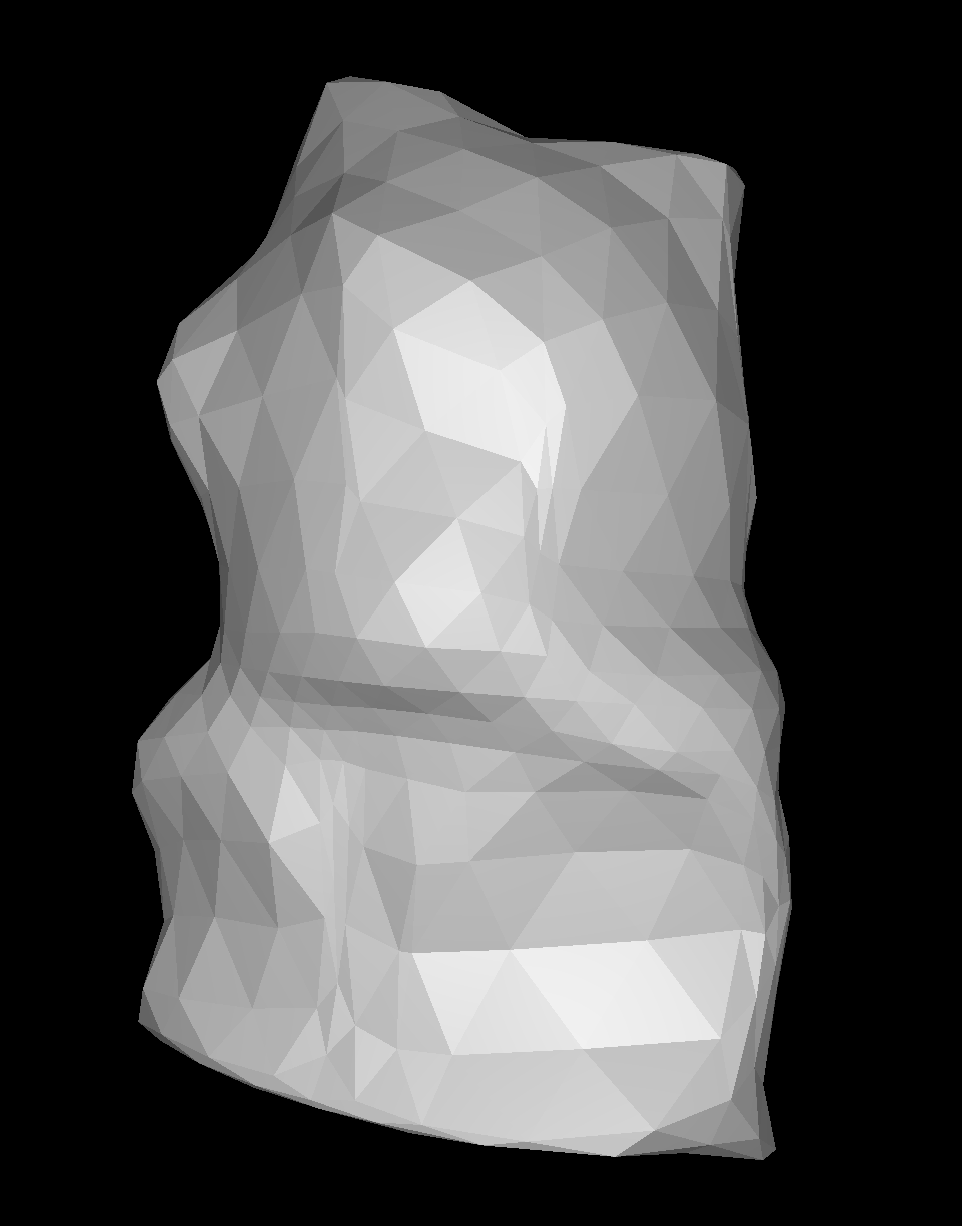
\includegraphics[width=\textwidth]{images/teddyfailure.png}
    \caption{Lack of detail}
    \label{teddyfailure}
  \end{subfigure}
  \caption{Lack of detail when attempting to fit to larger targets with many folds}
  \label{teddytarget}
\end{figure}

\subsection{Implementation Details}

\subsubsection{Data Pipeline: Pranav Talluri}
\label{section:datapipe}

The original dataset uses images and viewpoint parameters from ShapeNet stored in NumPy array files as inputs. To make the pipeline extensible, this is replaced with a folder input for images. The camera parameters can then be given according to the ground truth of the dataset or inferred from the images. This enables us to switch between data sources and image samples by simply editing the image source path. All input images are resized to 256x256 as this was found to be ideal for execution time for the fitting procedure.

We can place novel images that we captured in an input folder and then utilise camera parameter estimation or, if we know what angles we took the images from, ground truth data. Figure \ref{natdatapipe} shows the data pipeline when we utilise novel images.

\begin{figure}[h!]
  \centering
  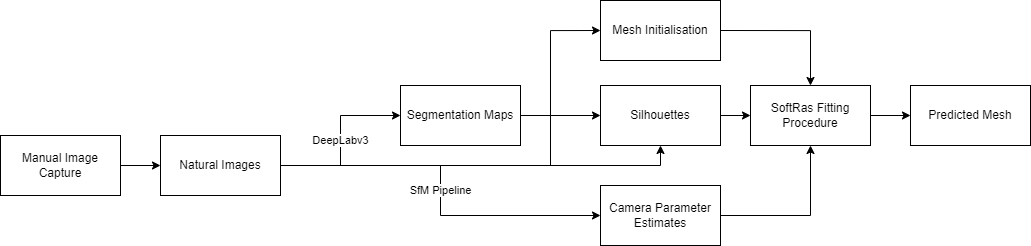
\includegraphics[width=\textwidth]{images/natdatapipeline.png}
  \caption{Data pipeline for newly captured images}
  \label{natdatapipe}
\end{figure}

The ALOI dataset images are taken every 5 degrees in a complete rotation around the object. The camera parameters can be inferred from this information. The code used to perform this initialisation is shown in Figure \ref{camerainitaloi}.

\begin{figure}[h!]
  \centering
  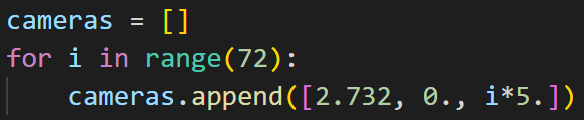
\includegraphics[width=0.35\textwidth]{images/initcamera.png}
  \caption{Viewpoint parameter initialisation for ALOI}
  \label{camerainitaloi}
\end{figure}

The ALOI dataset also comes with ground truth object/background binary masks, which we utilise to generate silhouettes from the raw images. This is shown in Figure \ref{datapipeline}. We experimented with grey-scale and colour silhouettes and found no difference in results (as colour is not considered in the loss computation), so we converted the silhouettes to grey scale. Figure \ref{aloidatapipe} shows the new data pipeline for testing using the ALOI dataset.

\begin{figure}[h!]
  \centering
  \begin{subfigure}{0.23\textwidth}
    \centering
    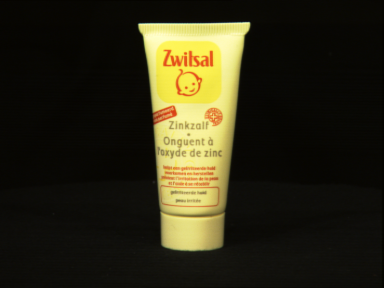
\includegraphics[width=\textwidth]{images/moisturiserpng.png}
    \caption{Original image (384 x 288)}
    \label{moistpng}
  \end{subfigure}
  \hfill
  \begin{subfigure}{0.23\textwidth}
    \centering
    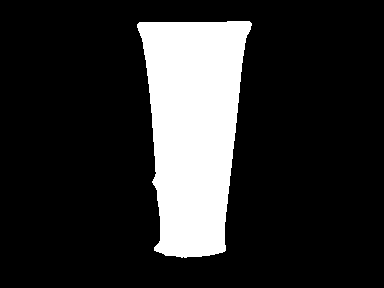
\includegraphics[width=\textwidth]{images/moisturisermask.png}
    \caption{Ground truth mask (384 x 288)}
    \label{moistmask}
  \end{subfigure}
  \hfill
  \begin{subfigure}{0.23\textwidth}
    \centering
    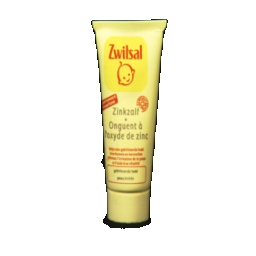
\includegraphics[width=\textwidth]{images/moisturisersil.png}
    \caption{Generated silhouette (256x256)}
    \label{moistsil}
  \end{subfigure}
  \hfill
  \begin{subfigure}{0.23\textwidth}
    \centering
    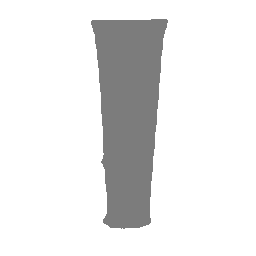
\includegraphics[width=\textwidth]{images/moisturisersilgrey.png}
    \caption{Generated silhouette grey-scale (256x256)}
    \label{moistsilgrey}
  \end{subfigure}
  \caption{Image pipeline for ALOI}
  \label{datapipeline}
\end{figure}

\begin{figure}[h!]
  \centering
  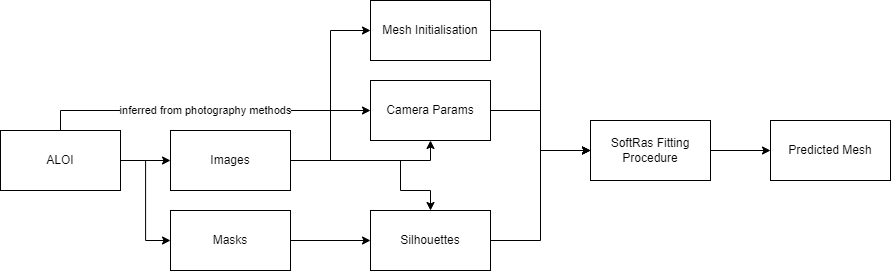
\includegraphics[width=\textwidth]{images/aloidatapipe.png}
  \caption{Data pipeline using ALOI dataset}
  \label{aloidatapipe}
\end{figure}

\newpage
\subsubsection{Silhouette Initialisation: Pranav Talluri}

As stated in \ref{section:silimp}, we estimate silhouettes for natural images using segmentation. We run DeepLab on the input images and use the segmentation masks as binary object/background masks, which we can add to the image as an $\alpha$ channel. This is performed in the segment.py module as shown in Figure \ref{segment}. 

\begin{figure}[h!]
  \centering
  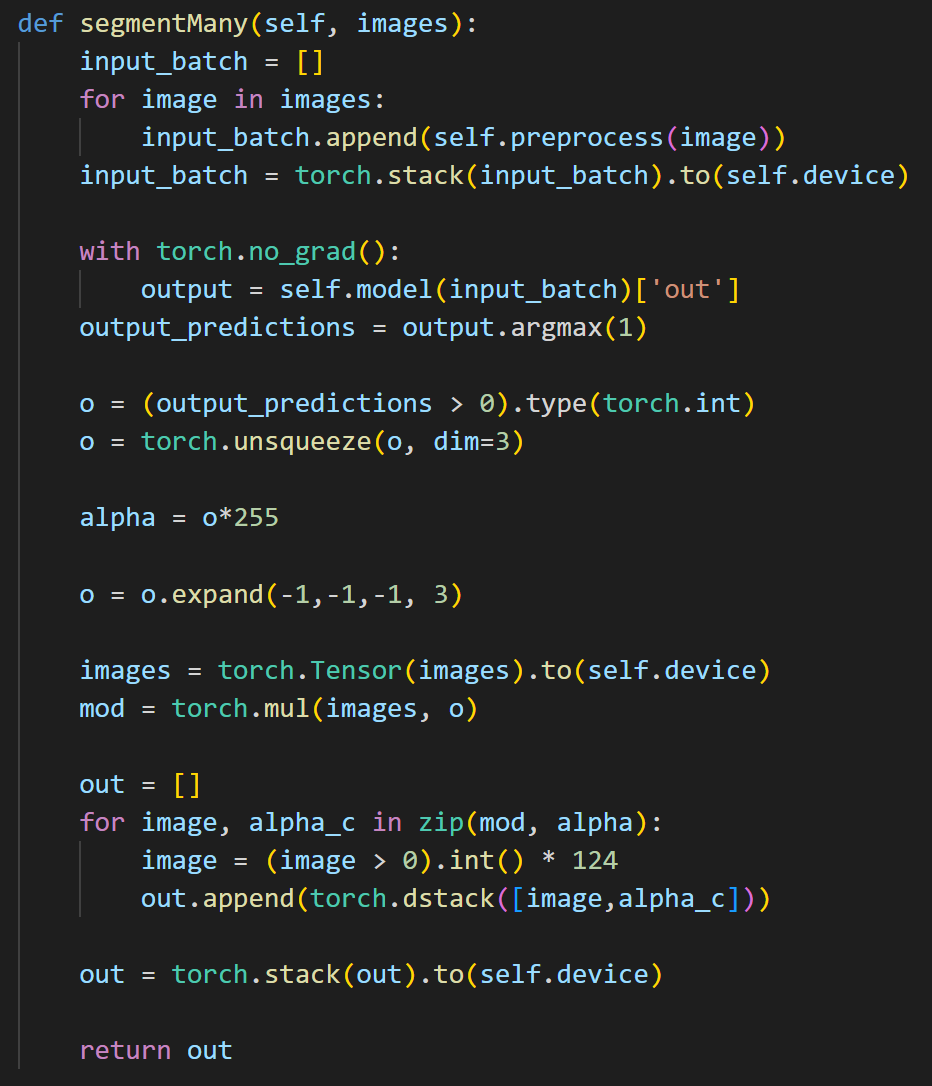
\includegraphics[width=0.5\textwidth]{images/segmentcode.png}
  \caption{Code used to perform segmentation using DeepLabv3}
  \label{segment}
\end{figure}

\newpage
\subsubsection{Mesh Initialisation: Pranav Talluri}
\label{section:meshinitcode}

We create higher polygon count sphere initialisations in Blender using a simple UV sphere and the subdivide functionality. The straightforward process is shown if Figure \ref{blender}. We also modify the SoftRas pipeline to deal with 256x256 images, which is a simple parameter change when initialising the soft rasteriser during the fitting procedure.

\begin{figure}[h!]
  \centering
  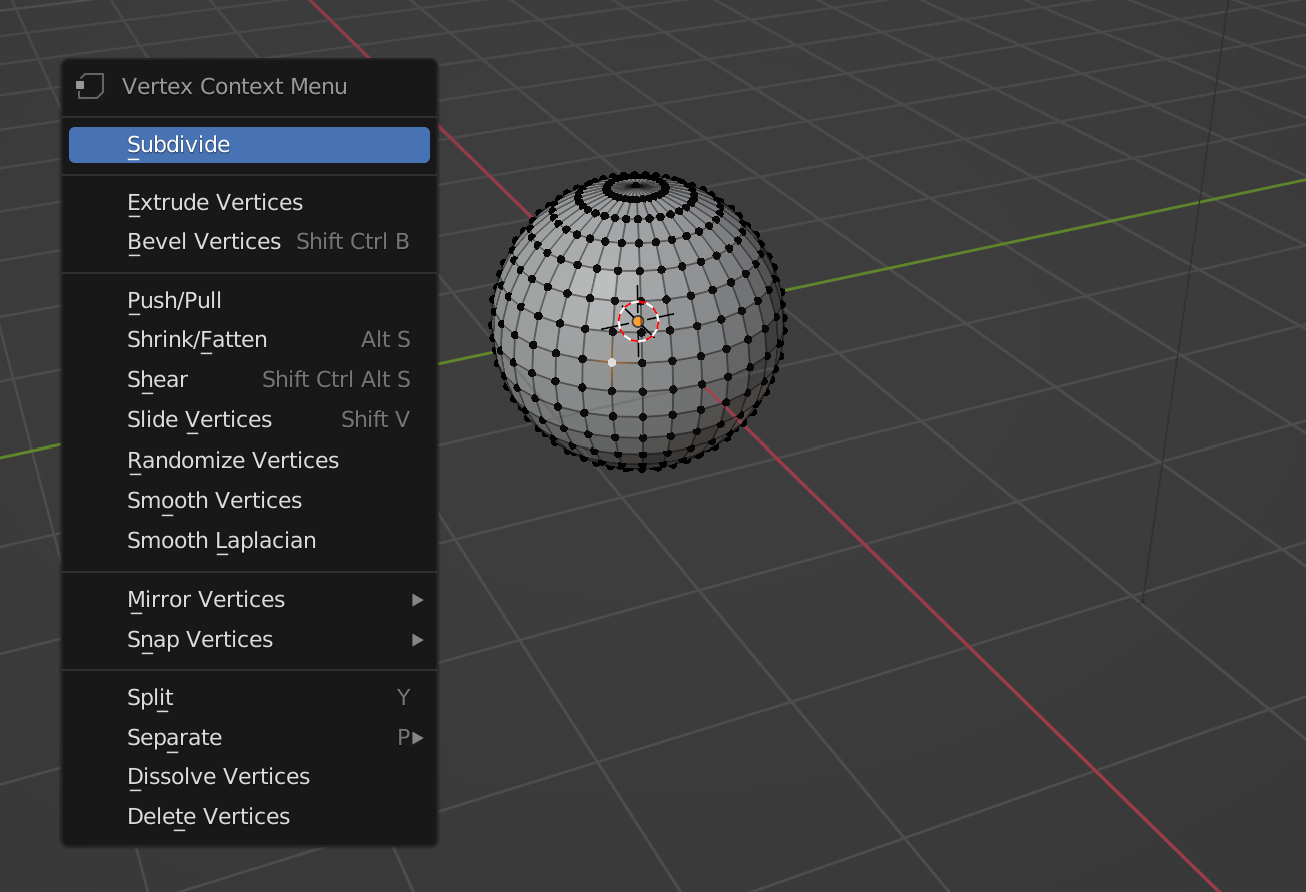
\includegraphics[width=0.4\textwidth]{images/blender.png}
  \caption{Creating higher polygon count spheres in Blender}
  \label{blender}
\end{figure}

In order to modify this mesh according to the target object, we first examine an image of the target object as shown in Figure \ref{imageeval}. This gives us the height and width of the object in pixels, as well as the top and left of the object in terms of the image dimensions. The code for these mesh modifications is found in init\_mesh.py.

\begin{figure}[h!]
  \centering
  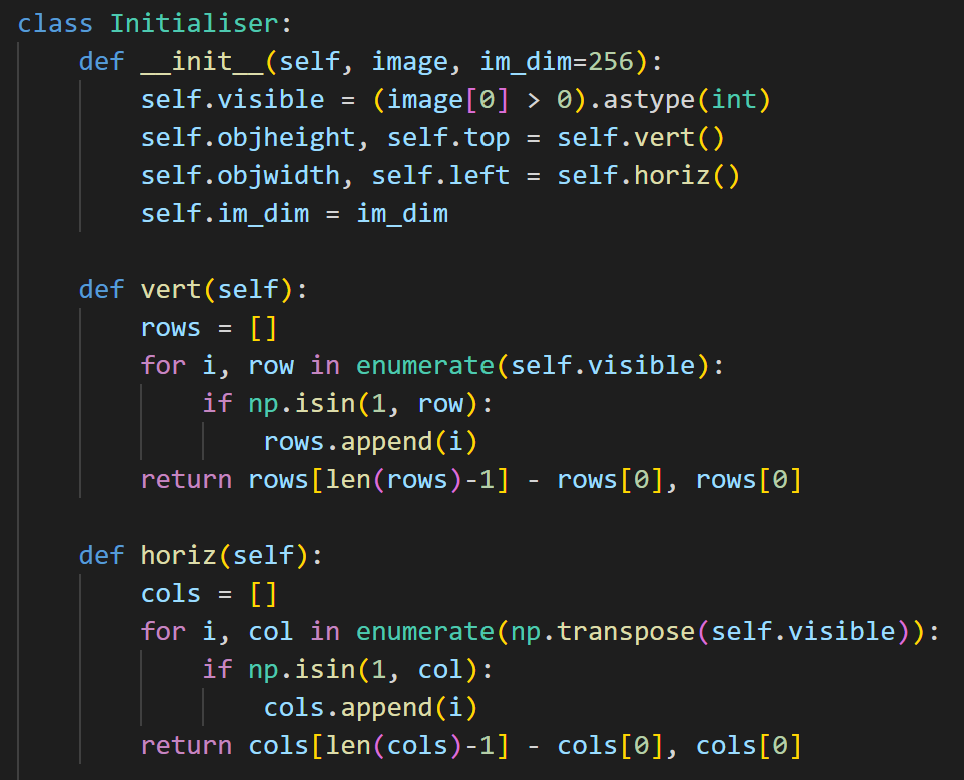
\includegraphics[width=0.5\textwidth]{images/image_eval.png}
  \caption{Inferring information about the target object from a target image}
  \label{imageeval}
\end{figure}

The first step is to scale the $x$ and $y$ dimensions of the sphere according the the aspect ratio and size of the target object. The code for this is shown in Figure \ref{scalecode}.

\begin{figure}[h!]
  \centering
  \begin{subfigure}{0.55\textwidth}
    \centering
    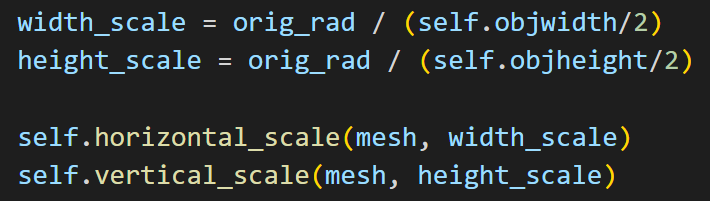
\includegraphics[width=\textwidth]{images/scale_a.png}
    \caption{Calculate the scale factors}
  \end{subfigure}
  \hfill
  \begin{subfigure}{0.4\textwidth}
    \centering
    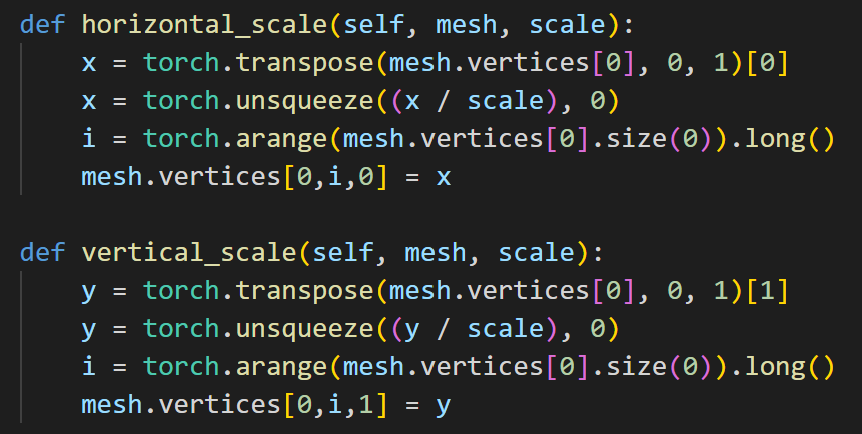
\includegraphics[width=\textwidth]{images/scale_b.png}
    \caption{Scale the mesh accordingly}
  \end{subfigure}
  \caption{Scaling the initial mesh according to the target object}
  \label{scalecode}
\end{figure}

We can then shift the initial mesh according to where in the 256x256 image the target object is. The code for this is shown in Figure \ref{shiftcode}.

\begin{figure}[h!]
  \centering
  \begin{subfigure}{0.55\textwidth}
    \centering
    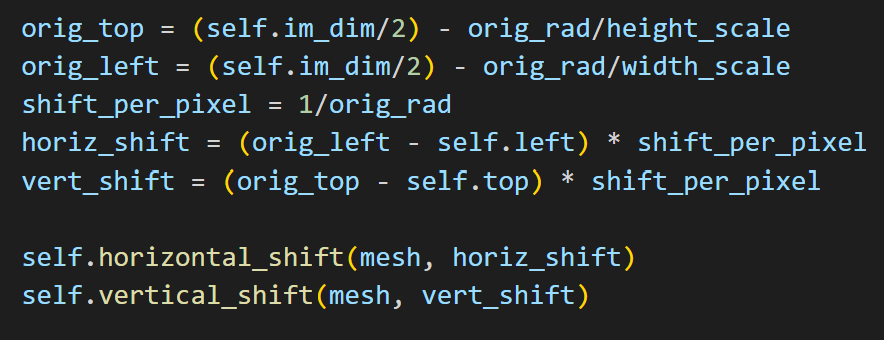
\includegraphics[width=\textwidth]{images/shift_a.png}
    \caption{Calculate the shift amounts}
  \end{subfigure}
  \hfill
  \begin{subfigure}{0.4\textwidth}
    \centering
    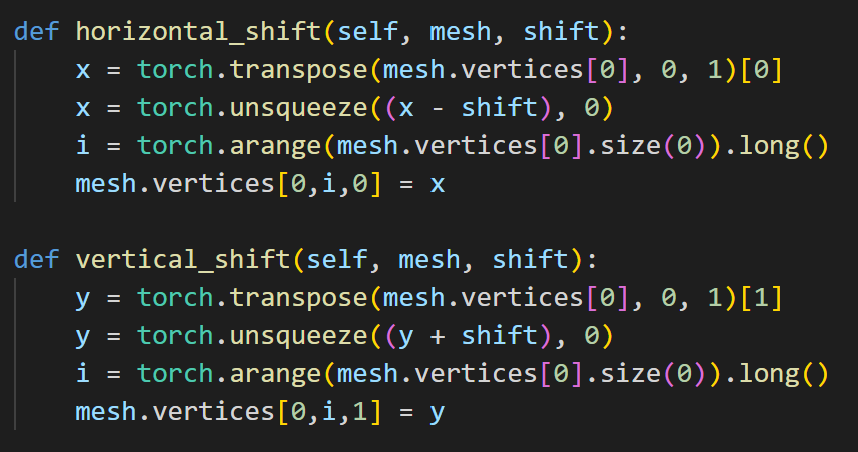
\includegraphics[width=\textwidth]{images/shift_b.png}
    \caption{Shift the mesh accordingly}
  \end{subfigure}
  \caption{Translating the initial mesh according to the target object}
  \label{shiftcode}
\end{figure}

\newpage
\subsection{Fitting Procedure: Pranav Talluri}

The fitting procedure is relatively unchanged. We still use the Adam optimiser to optimise the negative IoU loss between renders of the target image and the ground truth target image. The function used to compute the loss is shown in Figure \ref{lossfitting}. The original paper uses $\beta = (0.9, 0.999)$, however, we found that $\beta = (0.5, 0.99)$ produces better results, qualitatively and quantitatively, in practice. Figure \ref{initfitting} shows this and the other initialisations made. The code for the fitting procedure is given in build\_mesh.py. The code iterated in each loop to improve the mesh is shown in Figure \ref{iterfitted}.

\begin{figure}[h!]
  \centering
  \begin{subfigure}{.7\textwidth}
    \centering
    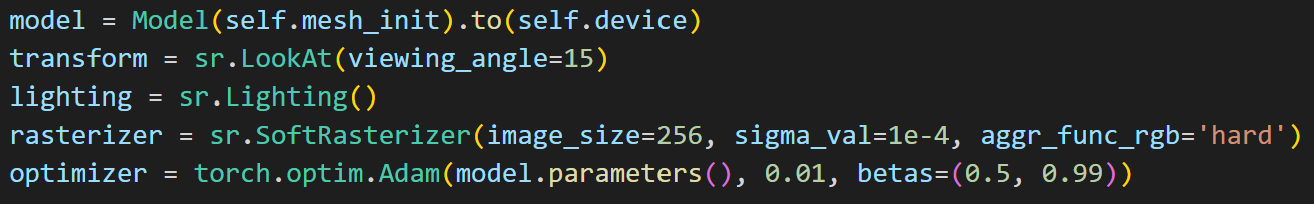
\includegraphics[width=\textwidth]{images/fittingcode_a.png}
    \caption{Set up model and initialisation}
    \label{initfitting}
  \end{subfigure}
  \hfill
  \begin{subfigure}{.7\textwidth}
    \centering
    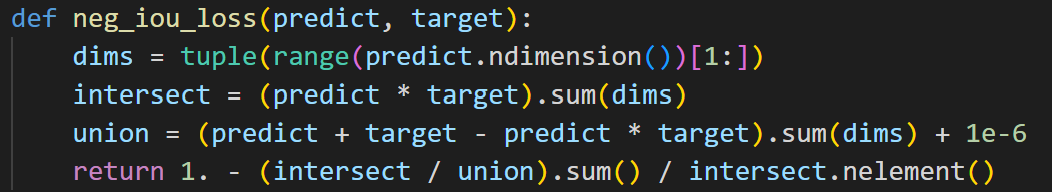
\includegraphics[width=\textwidth]{images/fittingcode_b.png}
    \caption{Loss computation}
    \label{lossfitting}
  \end{subfigure}
  \hfill
  \begin{subfigure}{.7\textwidth}
    \centering
    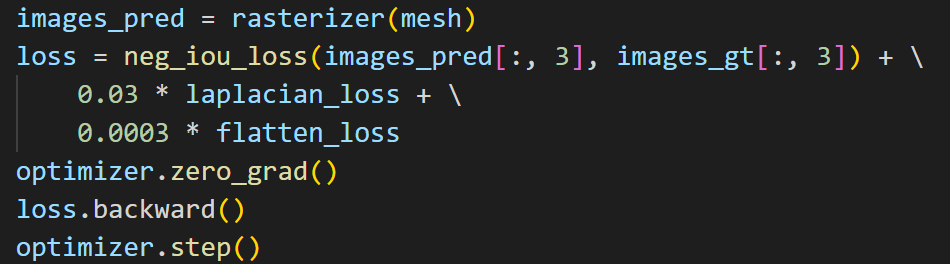
\includegraphics[width=\textwidth]{images/fittingcode_c.png}
    \caption{Iterated code}
    \label{iterfitted}
  \end{subfigure}
  \caption{Code for fitting procedure}
  \label{fittingcode}
\end{figure}

\newpage
\section{Experiments and Evaluation}
\subsection{Datasets}

\subsubsection{ALOI and ShapeNet: Pranav Talluri}

ALOI is the main dataset that we use to test and evaluate the performance of the fitting procedure. It consists of photo-realistic images of small objects taken from 72 angles. This is in contrast to the dataset used by the original paper's authors, ShapeNet, which consists of rendered images of very simple computer generated models from multiple angles and multiple elevations. We still perform some testing on ShapeNet, specifically to verify the benefits of mesh initialisation. Samples from ALOI are shown in Figure \ref{aloisamples} and samples from ShapeNet are shown in Figure \ref{shapenetinput}.

The reasons we chose to use ALOI in our investigations align with the differences between it and ShapeNet. We wanted to explore whether SoftRas was capable of fitting objects when given high-detail, photo-realistic images. The lack of multiple elevations was also an interesting test to see whether SoftRas could reconstruct appropriate meshes given variation in only two axes. In reality, the lack of multiple elevations was causes issues for some of the objects. Specifically, when an object has internal folds (i.e., a concave structure), without vertical angles, there is no way for SoftRas to identify the structure.

Most importantly, the added challenge in the ALOI dataset further highlights the need for auto-initialising the other parameters in order to achieve good reconstruction results.

As well as testing on ALOI, we perform some testing on natural images that we captured ourselves. This highlights the improvement in functionality that our initialisations enable. Specifically that the silhouettes and camera parameters of natural images can be estimated before the fitting procedure, improving the compatibility of the fitting procedure with far more data.

\subsubsection{Natural Images: Pranav Talluri}

This data is the most challenging for the pipeline for multiple reasons. 

Firstly, the success of the pipeline depends on successful segmentation of images from every viewpoint of the object. This is possible in our current pipeline but testing has highlighted the need for retraining DeepLabv3 on a more suitable dataset in order to segment backgrounds from small objects with simple backgrounds.

Next, the estimation of camera parameters introduces another source of inaccuracy in the reconstruction, based on how well the viewpoints can be inferred using the SfM pipeline.

Finally, compared to large-scale datasets like ALOI, the natural images we capture are likely to have more inaccuracy in alignment, as well as more variability in lighting and viewpoints.

\newpage
\subsection{Silhouette Initialisation: Pranav Talluri}

We test whether our silhouette generation pipeline works on novel, natural images that we capture. We perform two tests: on images of a bottle, and images of a potted plant.

The segmentation on the bottle performs quite well. With the vast majority of the 72 viewpoints getting good silhouettes. Occasionally, a silhouette will pick up elements from the table as shown in Figure \ref{bottleseg}. Also, the boundaries could be a bit tighter to the bottle.

\begin{figure}[h!]
  \centering
  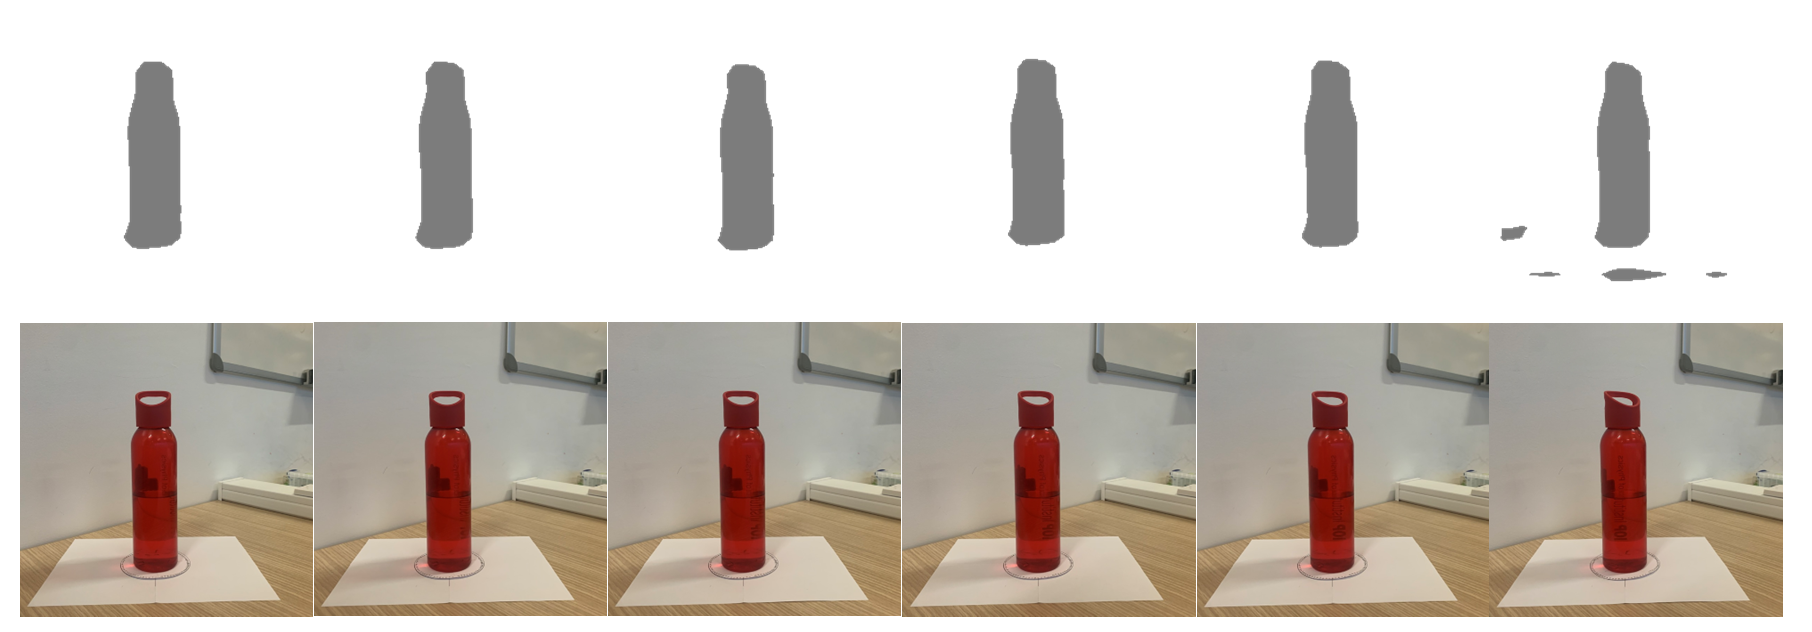
\includegraphics[width=\textwidth]{images/bottleseg.png}
  \caption{Segmentation performance on natural images of a water bottle}
  \label{bottleseg}
\end{figure}

The segmentation on the pot also performs well as shown in Figure \ref{natpotseg}. It also appears that having a more even table below the object, unlike the with the water bottle where there was a piece of paper, makes it less likely that the table is picked up as the foreground.

\begin{figure}[h!]
  \centering
  \begin{subfigure}{.35\textwidth}
    \centering
    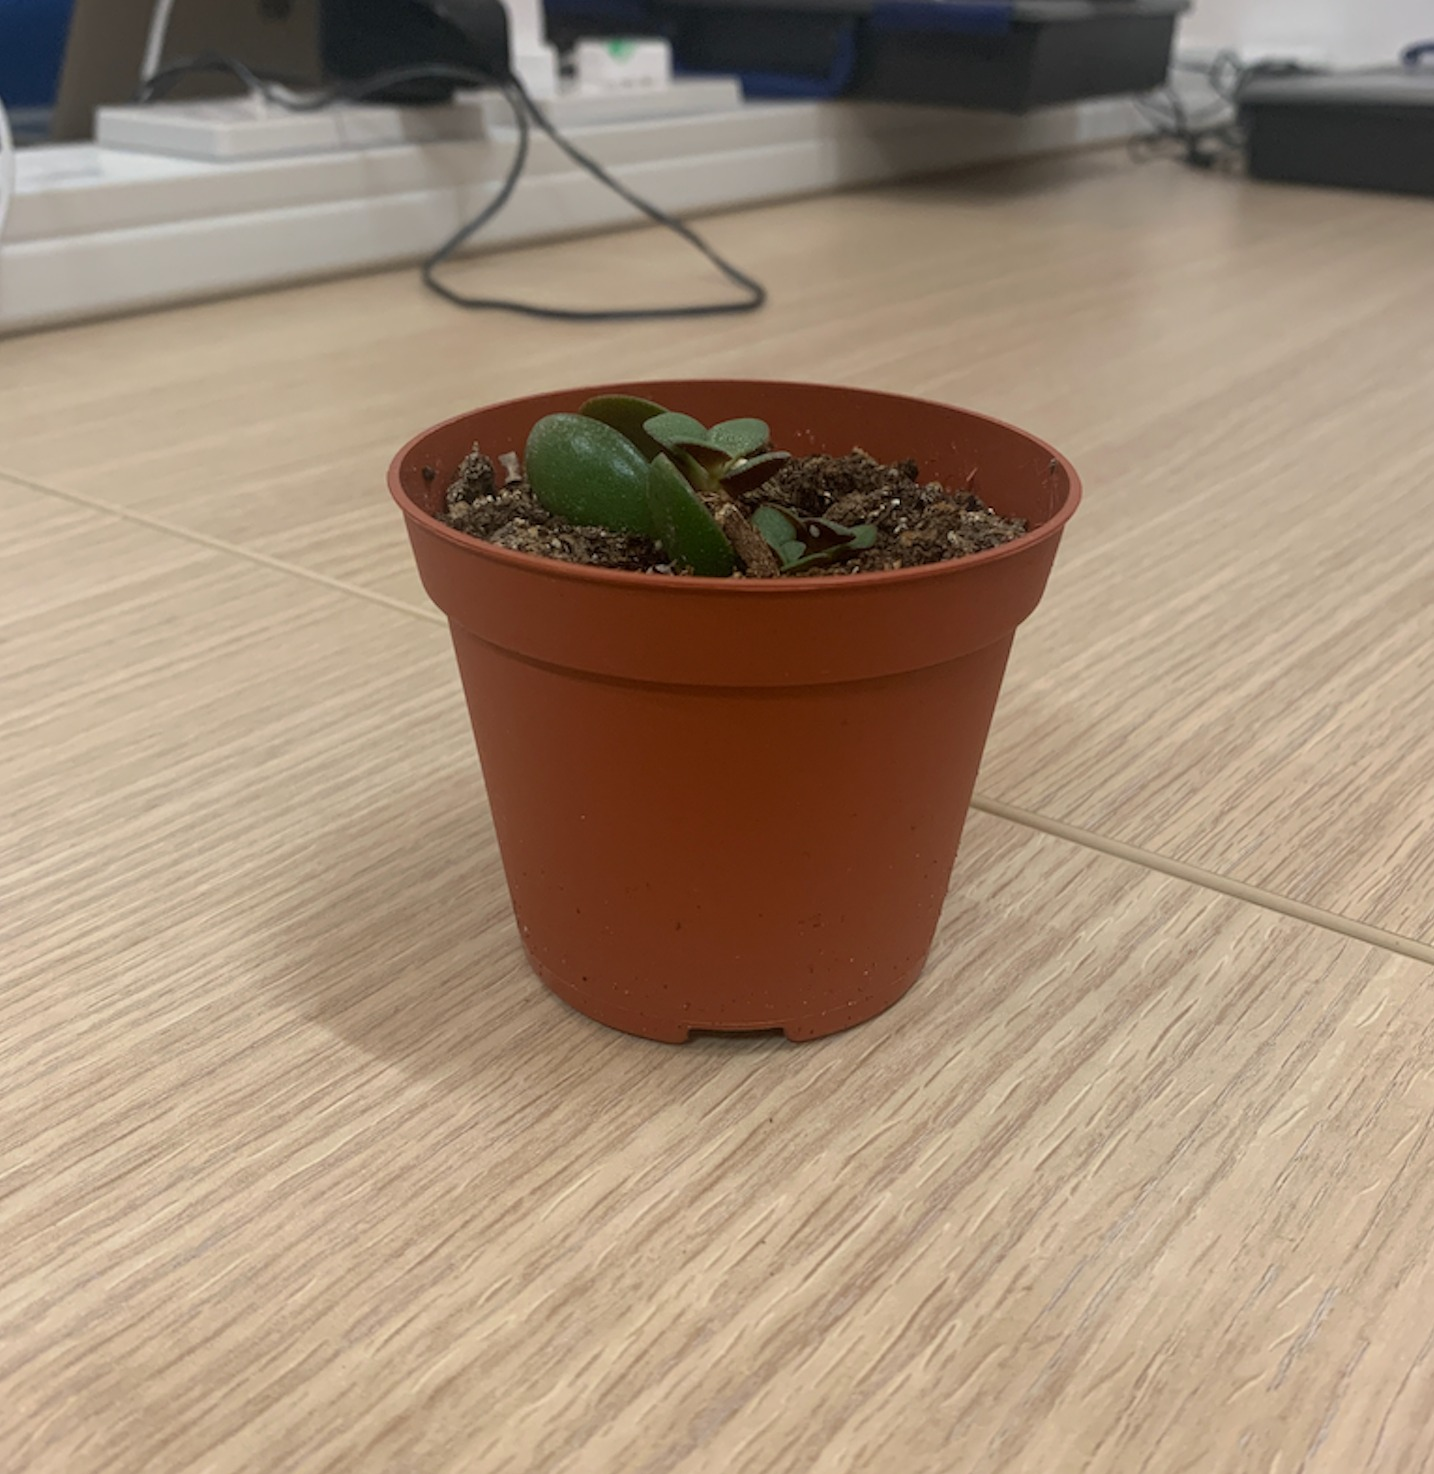
\includegraphics[width=\textwidth]{images/natpotpng.jpg}
    \caption{Plant pot}
    \label{natpotpng}
  \end{subfigure}
  \hfill
  \begin{subfigure}{.35\textwidth}
    \centering
    
\includegraphics[width=\textwidth]{images/natpotseg.png}
    \caption{Silhouette}
    \label{natpotsil}
  \end{subfigure}
  \caption{Silhouette estimation for natural image of plant pot}
  \label{natpotseg}
\end{figure}

\newpage
\subsection{Mesh Initialisation: Pranav Talluri}

We explore results for various objects from ShapeNet, ALOI and natural images with and without the initialisation detailed in Section \ref{section:meshinitcode}. Quantitatively, we can compare the losses of the various experiments. Qualitatively, we can compare the quality of the meshes produced.

\subsubsection{ALOI: Pranav Talluri}
\paragraph{Pot}
The first result we explore is a pot from ALOI. We examine the results of the fitting procedure without any mesh initialisation, with initialisation and also with a higher polygon count sphere.

Quantitatively, the loss over iterations suggests that the mesh initialisations we make are successful. Specifically, the initialised mesh converges to the same loss much faster and more stably than an uninitialised mesh. The performance between the high polygon count and low polygon count meshes appears the same.

Qualitatively, we see results in line with the losses. Initialising the mesh removes the artefacts we have at the top of the pot from the uninitialised mesh. This is likely due to the fact that the pot is in the bottom half of the frame and the fitting procedure no longer has to move and scale the mesh as much. Furthermore, using the higher polygon count mesh reduces the rotational artefacts as well. We hypothesis that with an even higher polygon count mesh, we would obtain a result without any twisting artefacts.

\begin{figure}[h!]
  \centering
  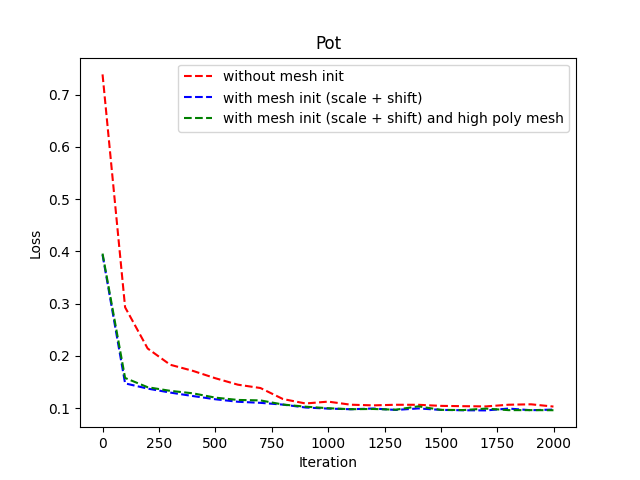
\includegraphics[width=0.6\textwidth]{images/potplot.png}
  \caption{Quantitative comparison between mesh initialisations for a pot}
  \label{results-pot-loss}
\end{figure}

\begin{figure}[h!]
  \centering
  \begin{subfigure}{.2\textwidth}
    \centering
    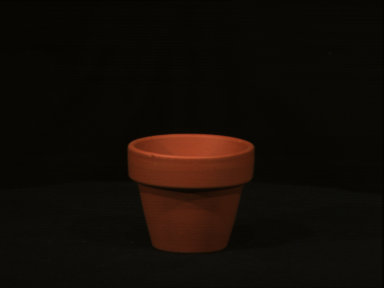
\includegraphics[width=\textwidth]{images/potpng.png}
    \caption{Target}
    \label{results-pot-mesh1}
  \end{subfigure}
  \hfill
  \begin{subfigure}{.2\textwidth}
    \centering
    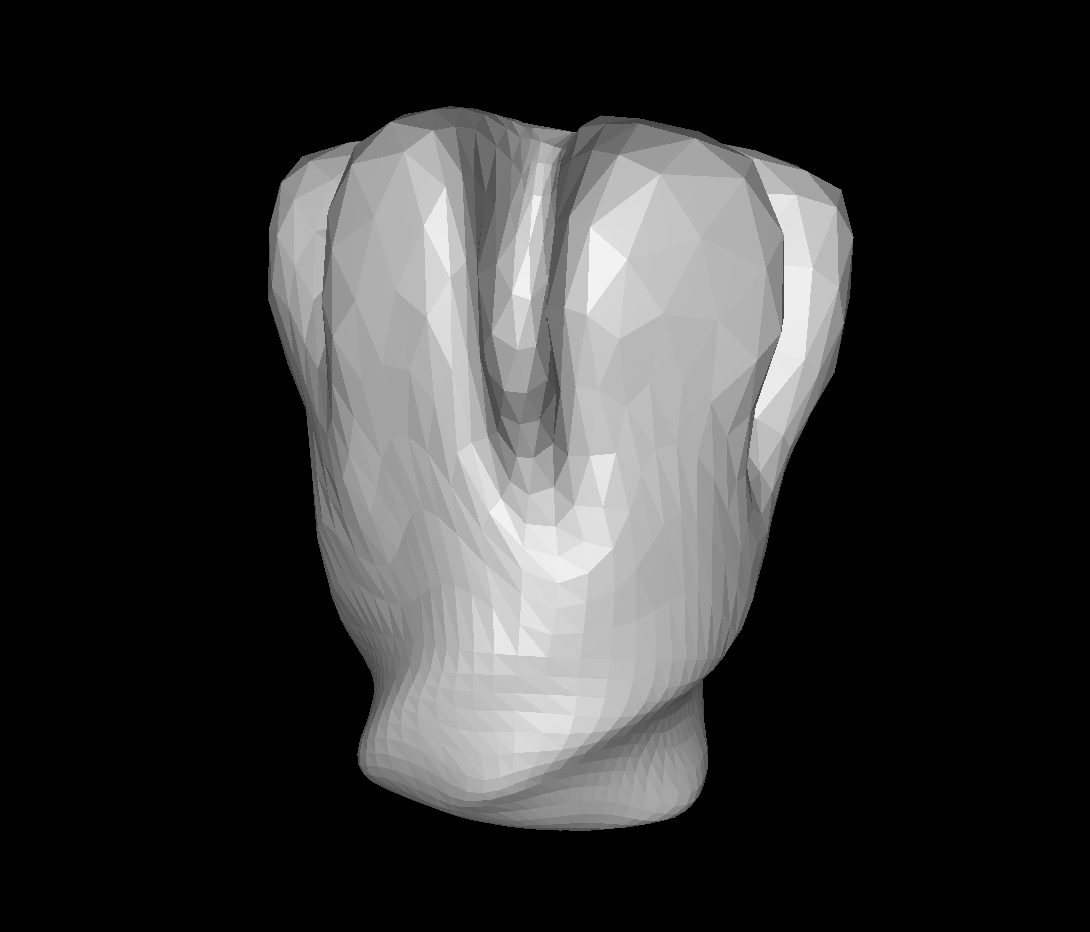
\includegraphics[width=\textwidth]{images/potmesh_a.png}
    \caption{No mesh initialisation}
    \label{results-pot-mesh2}
  \end{subfigure}
  \hfill
  \begin{subfigure}{.2\textwidth}
    \centering
    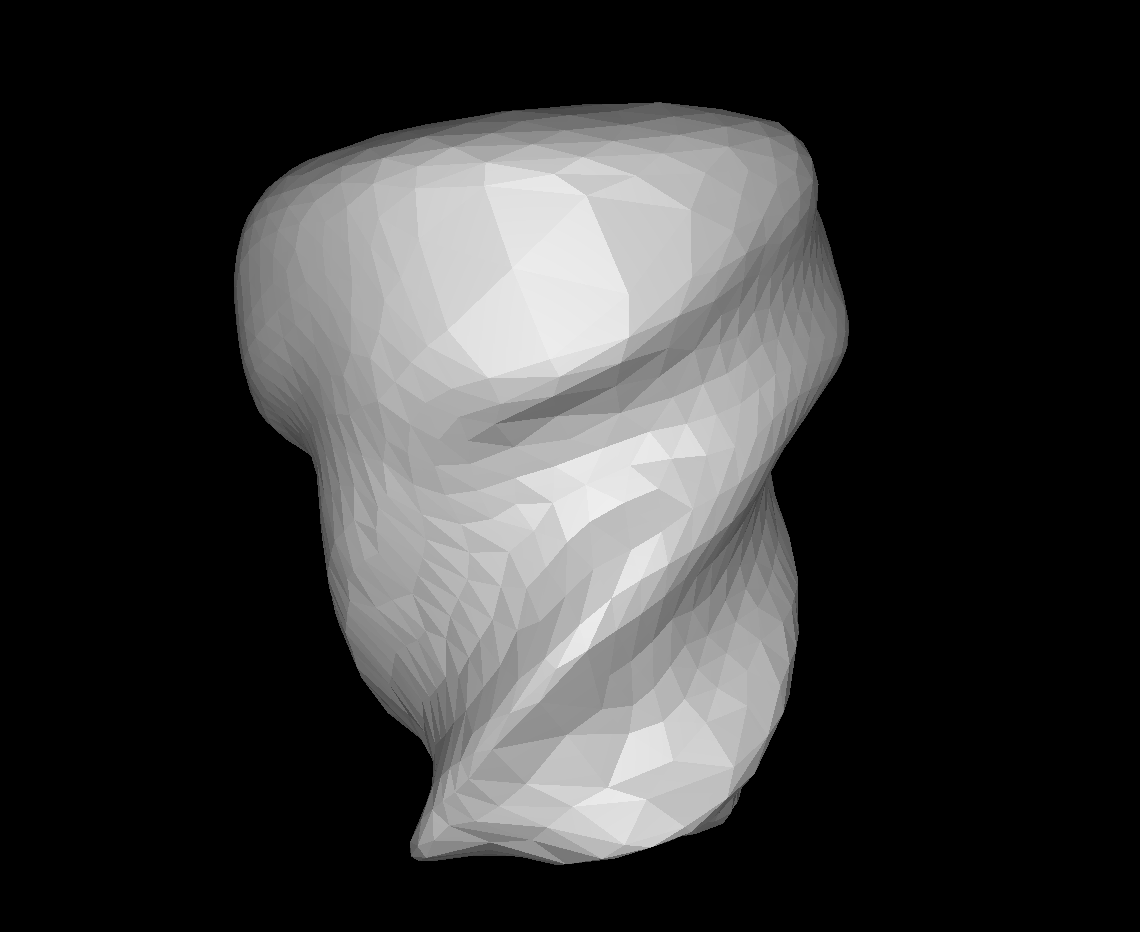
\includegraphics[width=\textwidth]{images/potmesh_b.png}
    \caption{Mesh initialisation (scale and shift)}
    \label{results-pot-mesh3}
  \end{subfigure}
  \hfill
  \begin{subfigure}{.2\textwidth}
    \centering
    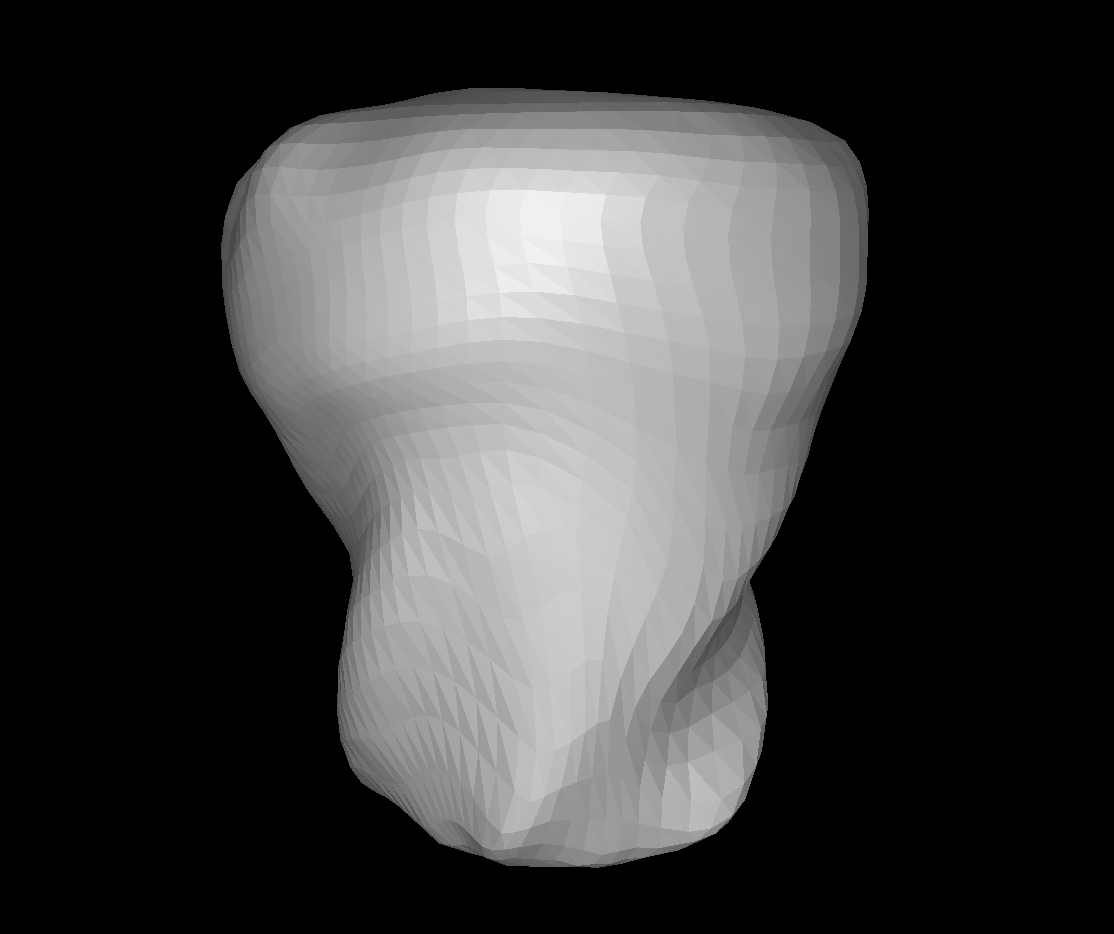
\includegraphics[width=\textwidth]{images/potmesh_c.png}
    \caption{Mesh init and high poly mesh}
    \label{results-pot-png}
  \end{subfigure}
  \caption{Qualitative comparison between mesh initialisations for a pot}
  \label{results-pot}
\end{figure}

\newpage
\paragraph{Moisturiser}
Next, we examine the results for a moisturiser bottle in ALOI under the same three initialisations as the pot.

This time, the initialised mesh appears to perform worse quantitatively. i.e., the loss converges slower than with the uninitialised mesh. Although this is somewhat mitigated with the higher polygon count initial mesh. We hypothesise that this is due to the scaling of the sphere not coinciding with the shape of the bottle. Specifically, scaling the sphere to the aspect ratio of the bottle produces a vertically stretched sphere, which thins at the top and bottom. However, the bottle is just as thick at the bottom as it is in the centre and even thicker at the top. This means extra iterations are required to shift the volume of the bottle towards these edges.

Qualitatively, the initialised mesh performs the same as, if not worse than the uninitialised mesh, with both of the results suffering from twisting artefacts. However, the higher polygon count mesh rectifies this and produces a very high quality reproduction of the target object. This is likely due to the fact that introducing more vertices makes it easier for the fitting procedure to create the required cylindrical shape at the bottom of the mesh, where the initialisation simply ends in a point.

\begin{figure}[h!]
  \centering
  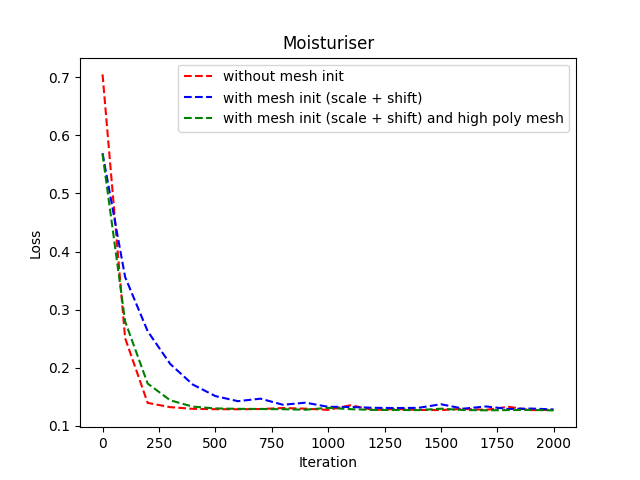
\includegraphics[width=0.6\textwidth]{images/moisturiserplot.png}
  \caption{Quantitative comparison between mesh initialisations for a moisturiser bottle}
  \label{results-moisturiser-loss}
\end{figure}

\begin{figure}[h!]
  \centering
  \begin{subfigure}{.2\textwidth}
    \centering
    \includegraphics[width=\textwidth]{images/moisturiserpng.png}
    \caption{}
    \label{results-moisturiser-mesh1}
  \end{subfigure}
  \hfill
  \begin{subfigure}{.2\textwidth}
    \centering
    \includegraphics[width=\textwidth]{images/moistmesh_a.png}
    \caption{No mesh initialisation}
    \label{results-moisturiser-mesh2}
  \end{subfigure}
  \hfill
  \begin{subfigure}{.2\textwidth}
    \centering
    \includegraphics[width=\textwidth]{images/moistmesh_b.png}
    \caption{Mesh initialisation (scale and shift)}
    \label{results-moisturiser-mesh3}
  \end{subfigure}
  \hfill
  \begin{subfigure}{.2\textwidth}
    \centering
    \includegraphics[width=\textwidth]{images/moistmesh_c.png}
    \caption{Mesh and high poly mesh}
    \label{results-moisturiser-png}
  \end{subfigure}
  \caption{Qualitative comparison between mesh initialisations for a moisturiser bottle}
  \label{results-moisturiser}
\end{figure}

\newpage
\paragraph{Apricot}

Next we examine an apricot from the ALOI dataset. This example was one of the motivating factors for the initialisation method, given the failure modes exhibited without any initialisation due to the size and location of the object in the frame.

Quantitatively, the mesh initialisation not only improves the speed of convergence, but also results in a better loss. We also see that using a lower polygon count initial mesh leads to further improvements in convergence time and the sample quality.

This is likely due to the fact that, as previously mentioned, when we have a small off-centre object, it is difficult for the fitting procedure to move and scale the mesh quickly and without introducing artefacts. We can see in the images of the meshes, that without an initialisation, the fitting procedure completely fails, resulting in a separation of the mesh. We hypothesise that this occurs due to the distance between the top of the mesh and the object, resulting in a lack of gradient to improve upon. This is rectified by the scaling and shifting of the mesh. Not that the shift is required when we scale here because otherwise, due to the size of the object, there would no longer be any overlap between the mesh and the image, resulting in a lack of gradient to optimise over. We also hypothesised that a lower polygon mesh would work better due to the size of the image and the artefacts found on the standard initialisation. Specifically, the excess material on the size of the mesh. In practice, we found that allowing the procedure to run for more iterations eventually results in this extra material being absorbed into the main shape, giving better qualitative results.

\begin{figure}[h!]
  \centering
  \includegraphics[width=0.6\textwidth]{images/apricotplot.png}
  \caption{Quantitative comparison between mesh initialisations for an apricot}
  \label{results-apricot-loss}
\end{figure}

\begin{figure}[h!]
  \centering
  \begin{subfigure}{.2\textwidth}
    \centering
    \includegraphics[width=\textwidth]{images/apricot.png}
    \caption{Target}
    \label{results-apricot-mesh1}
  \end{subfigure}
  \hfill
  \begin{subfigure}{.2\textwidth}
    \centering
    \includegraphics[width=\textwidth]{images/apricotmesh_a.png}
    \caption{No mesh initialisation}
    \label{results-apricot-mesh2}
  \end{subfigure}
  \hfill
  \begin{subfigure}{.2\textwidth}
    \centering
    \includegraphics[width=\textwidth]{images/apricotmesh_b.png}
    \caption{Mesh initialisation (scale and shift)}
    \label{results-apricot-mesh3}
  \end{subfigure}
  \hfill
  \begin{subfigure}{.2\textwidth}
    \centering
    \includegraphics[width=\textwidth]{images/apricotmesh_c.png}
    \caption{Mesh init and low poly mesh}
    \label{results-apricot-png}
  \end{subfigure}
  \caption{Qualitative comparison between mesh initialisations for an apricot}
  \label{results-apricot}
\end{figure}

\newpage
\paragraph{Teddy Bear}
Finally from the ALOI dataset, we examine a teddy bear. The key difficulty in this reconstruction, which highlights a drawback of the ALOI dataset is that SoftRas will never be able to construct the concave area between the teddy's legs without images taken from higher or lower elevations as the structure is not visible with a silhouette. This means that, although reconstructions are better with the changes to the mesh initialisation that we have made, they still do not perfectly resemble the original image.

\begin{figure}[h!]
  \centering
  \begin{subfigure}{.3\textwidth}
    \centering
    \includegraphics[width=\textwidth]{images/teddy.png}
    \caption{Target}
    \label{results-teddy-png}
  \end{subfigure}
  \hfill
  \begin{subfigure}{.3\textwidth}
    \centering
    \includegraphics[width=\textwidth]{images/teddyfailure.png}
    \caption{No mesh initialisation}
    \label{results-teddy-mesh1}
  \end{subfigure}
  \hfill
  \begin{subfigure}{.3\textwidth}
    \centering
    \includegraphics[width=\textwidth]{images/teddybetter.png}
    \caption{Mesh initialisation (scale and shift)}
    \label{results-teddy-mesh2}
  \end{subfigure}
  \caption{Qualitative comparison between mesh initialisations for a teddy bear}
  \label{results-teddy}
\end{figure}

\newpage
\subsubsection{ShapeNet: Pranav Talluri}

We now examine examples from ShapeNet. We start with a recreation of the original pipeline, and then add the changes we made to the mesh initialisation and image scale.

\paragraph{Plane}
We examine the results on the airplane images. The original project performed very well on this example, producing a tight reconstruction without artefacts. The goal here is not to improve on these original results, but simply match the performance when the initialisation is used, while using less iterations. However, we found that increasing the resolution of the images and the polygon count of the mesh counteracts the effects of the mesh initialisation, which resulted in slower convergence in practice, as shown in Figure \ref{results-plane}. However, under a fair comparison, equal polygon counts and resolutions, we found our initialisation to lead to faster convergences in our experiments. We hypothesise that the render of the plane with the higher resolution, that uses the mesh initialisation, would eventually converge to the same result.

\begin{figure}[h!]
  \centering
  \includegraphics[width=0.6\textwidth]{images/planeplot.png}
  \caption{Quantitative comparison between mesh initialisations for a plane}
  \label{results-plane-loss}
\end{figure}

\begin{figure}[h!]
  \centering
  \begin{subfigure}{.3\textwidth}
    \centering
    \includegraphics[width=\textwidth]{images/airplanepng.png}
    \caption{Target}
    \label{results-plane-mesh1}
  \end{subfigure}
  \hfill
  \begin{subfigure}{.3\textwidth}
    \centering
    \includegraphics[width=\textwidth]{images/planemesh_a.png}
    \caption{No mesh initialisation - 64x64 input}
    \label{results-plane-mesh2}
  \end{subfigure}
  \hfill
  \begin{subfigure}{.3\textwidth}
    \centering
    \includegraphics[width=\textwidth]{images/planemesh_b.png}
    \caption{Mesh initialisation - 256 x 256 input}
    \label{results-plane-mesh3}
  \end{subfigure}
  \caption{Qualitative comparison between mesh initialisations for a plane}
  \label{results-plane}
\end{figure}

\newpage
\subsubsection{Natural Images: Pranav Talluri and Yujia Yang}
\paragraph{Bottle}

We test the mesh initialisation pipeline on natural images we captured of a water bottle. In this case, the mesh initialisation slows down the convergence to the final mesh. This is likely for the same reason as the moisturiser example from ALOI, where using a mesh initialisation with a taper at the top and the bottom is detrimental to convergence time for cylindrical objects. The qualitative results are impressive considering that they are a new feature of the pipeline, and hence have no previous results to compare with. It is notable that the twisting artefacts are present.

\begin{figure}[h!]
  \centering
  \includegraphics[width=0.6\textwidth]{images/bottleplot.png}
  \caption{Quantitative comparison between mesh initialisations for a bottle}
  \label{results-natbottle-loss}
\end{figure}

\begin{figure}[h!]
  \centering
  \begin{subfigure}{.2\textwidth}
    \centering
    \includegraphics[width=\textwidth]{images/natbottlepng.png}
    \caption{Target}
    \label{results-natbottle-target}
  \end{subfigure}
  \hfill
  \begin{subfigure}{.2\textwidth}
    \centering
    \includegraphics[width=\textwidth]{images/natbottlemesh_a.png}
    \caption{No mesh initialisation}
    \label{results-natbottle-mesh1}
  \end{subfigure}
  \hfill
  \begin{subfigure}{.2\textwidth}
    \centering
    \includegraphics[width=\textwidth]{images/natbottlemesh_b.png}
    \caption{Mesh initialisation (scale and shift)}
    \label{results-natbottle-mesh2}
  \end{subfigure}
  \caption{Qualitative comparison between mesh initialisations for a bottle}
  \label{results-natbottle}
\end{figure}

\newpage
\section{Conclusions and Future Directions}
\subsection{Conclusions: Pranav Talluri}

The main aims of this project were to:

\begin{enumerate}
  \item Improve the speed of convergence of shape-fitting of SoftRas using mesh auto-initialisations
  \item Improve the results of shape-fitting using mesh auto-initialisations
  \item Extend the functionality of shape-fitting using silhouette and camera parameter initialisation
\end{enumerate}

By this criteria, the project has been very successful.

The mesh initialisation performed identifies and addresses the weaknesses in the default initialisation used in the original code. This often improves the amount of time to converge taking the responsibility of position and scale of the mesh away from the fitting procedure and performing it faster and with lower likelihood of introducing artefacts.

Additionally, these changes often result in better outputs from the fitting procedure, either by mitigating the artefacts that would have otherwise been introduced in the shape fitting procedure, by utilising the extra iterations available due to the faster convergence, or because a successful fit was not originally possible (as in the case of the apricot \ref{results-apricot}).

Finally, the functionality and usability of the pipeline has been vastly improved. Originally, the fitting procedure would only accept inputs in the form of silhouettes and of a specific size. Now, due to the addition of the silhouette prediction layer and the auto-image resizing, the pipeline can accept images of any size and format and attempt to produce a mesh for a recognised object. This is vital in allowing the pipeline to be used in the real world where the ground truth silhouettes and masks are not known.

\subsection{Discussion of Limitations: Pranav Talluri}

\subsubsection{DeepLab for Silhouettes}

The first limitation we came across was utilising DeepLab for performing segmentation on natural images. Although DeepLab is very flexible in terms of its inputs, without proper training on the desired data types, it is not able to perform accurate segmentation. For example, attempts to perform segmentation on the data from ALOI rather than using the ground truth masks failed as DeepLab was not able to generalise to such a large variety of images and often would not detect any classes in the image.

\subsubsection{Mesh Initialisation Methods}

The second limitation was the methods we used for mesh initialisation. Although the methods used were very successful for most inputs and achieved our aims, they also highlighted some issues for some didactic examples. As previously discussed, utilising a stretched sphere is not ideal for cylindrical or cubical objects as the fitting procedure has to then shift volume from into the poles.

\subsubsection{Polygon Count and Iterations}

The final limitation was the limitation of computing power. We performed all testing on a single device, which meant we were limited by its performance. This meant we were not able to conduct extensive testing with even higher polygon counts or more iterations. From some initial testing, it seemed that adding more iterations could be used to give higher quality results when there were still unnecessary extrusions from the surface of the mesh.

\subsection{Future Directions: Pranav Talluri}

The future directions address the limitations of the current project. Especially for the mesh initialisations, there were many ideas that we hypothesise would have been useful, but we were not able to implement given the time constraints.
\begin{itemize}
  \item Retrain DeepLab on a new dataset that better reflects the objects that we are trying to reconstruct
  \item Detecting cylindrical target objects and using a cylinder mesh initialisation
  \item Currently, the sphere scaling only applies to two dimensions, considering another image orthogonal to the first would allow us to scale the third axis as well
  \item Detecting cubical target objects and using a cube mesh initialisation
  \item Using a more powerful machine such as the HPC to test with higher polygon count initialisations and with more iterations
  \item Use the silhouette estimations of images to generate a 3D mesh, i.e., convert the 2D silhouette into a 3D prism to act as the initialisation
\end{itemize}

\newpage
\section{Contributions}
\subsection{Pranav}

\begin{itemize}
  \item Pranav was responsible for bulding the fitting procedure pipeline. This is the main code from which other modules are called and is built to be extensible.

  \item Pranav was responsible for adapting the pipeline to new datasets, i.e., dealing with higher resolution inputs and image based inputs rather than NumPy inputs.
  
  \item Pranav implemented the silhouette generation for ALOI using the given masks by generating alpha channels for the standard RGB inputs.
  
  \item Pranav implemented DeepLabv3 for novel image silhouette estimation.
  
  \item Pranav built the mesh initialisation pipeline for selecting the initial mesh, and then scaling and transforming it according to the input image.
  
  \item Pranav generated figures and renders for inclusion in the paper and the presentation.
\end{itemize}

\subsection{Yujia}

\begin{itemize}
  \item Yujia captured the novel images to test in the pipeline.
\end{itemize}

\subsection{Ke}

\begin{itemize}
  \item Ke worked on camera parameter estiamtion using SfM in ColMap and MeshRoom.
\end{itemize}

\newpage
\printbibliography[
  heading=bibintoc,
  title={References}
]
\end{document}